\documentclass[11pt,a4,twosided,singlespacing,titlepagenumber=on]{scrreprt}

\usepackage[T1]{fontenc} % Handles accents etc better in the invisible details of the pdf output.
\usepackage[latin1]{inputenc} % May or may not be needed. Says that your *.tex file is a text file with ASCII latin1 encoding. You could use e.g. utf8 instead for easier accents etc.
\usepackage[UKenglish]{babel} % Let LaTeX know what language the text is in so it can select the correct hyphenation pattern etc

\newcommand{\Var}{\mathrm{Var}}

%%% American Mathematical Society packages
\usepackage{amsfonts,amssymb,amsmath,amsthm}
\usepackage{amsbsy}

\usepackage{listings}
\usepackage{color}

\definecolor{dkgreen}{rgb}{0,0.5,0}
\definecolor{gray}{rgb}{0.5,0.5,0.5}
\definecolor{mauve}{rgb}{0.58,0,0.82}

\definecolor{mygreen}{RGB}{28,172,0} % color values Red, Green, Blue
\definecolor{mylilas}{RGB}{170,55,241}

\lstset{
  frame=tblr,           
  language=R,
  otherkeywords={!,!=,~,$,\&,\%/\%,\%\%,<<-,_,/,*},
  deletekeywords={c, D, data, mean, cbind, hat, class, length, log, sum,
  col},
  aboveskip=5mm,
  belowskip=5mm,
  showstringspaces=false,
  columns=flexible,
  keepspaces=true,
  basicstyle={\small\ttfamily},
  backgroundcolor=\color{white}, 
  numbers=none,                      
  numberstyle=\tiny\color{gray},   
  keywordstyle=\color{blue},
  commentstyle=\color{dkgreen},
  stringstyle=\color{mauve},
  breaklines=true,              
  breakatwhitespace=true,
  tabsize=3,
}

\lstset{language=Matlab,%
    %basicstyle=\color{red},
    breaklines=true,%
    morekeywords={matlab2tikz},
    keywordstyle=\color{blue},%
    morekeywords=[2]{1}, keywordstyle=[2]{\color{black}},
    identifierstyle=\color{black},%
    stringstyle=\color{mylilas},
    commentstyle=\color{mygreen},%
    showstringspaces=false,%without this there will be a symbol in the places where there is a space
    numbers=left,%
    numberstyle={\tiny \color{black}},% size of the numbers
    numbersep=9pt, % this defines how far the numbers are from the text
    emph=[1]{for,end,break},emphstyle=[1]\color{red}, %some words to emphasise
    %emph=[2]{word1,word2}, emphstyle=[2]{style},    
}

%VERY USEFUL
\allowdisplaybreaks

\usepackage{algorithm}
\usepackage[noend]{algpseudocode}

%\usepackage{bm} % Possibly a better alternative to amsbsy for making bold typeface math.

%%% Graphics packages
\usepackage{graphicx}
\graphicspath{{img/}} % Useful if you have lots of images and want to keep thinks tidy by having a subfolder for images
%\usepackage{epstopdf} % If you produce your graphs as .eps files but then want to compile straight to PDF (e.g. because you are using TeXworks.) you may want to use this option. A better alternative of course would be to save all your graphs as *.pdf files from the start. Note that if you are compiling to pdf through PS/DVI then all your figures should be *.eps files and the epstopdf package should not be used.
%\usepackage{tikz} %For creating vector-graphics diagrams, flowcharts etc directly in LaTeX (takes some time to learn)
\usepackage[absolute]{textpos} % Used to position the Imperial College logo. You can comment this line and the next line out if you don't use the logo.
%\setlength{\TPHorizModule}{\paperwidth}\setlength{\TPVertModule}{\paperheight}
%\setlength{\TPHorizModule}{1cm}\setlength{\TPVertModule}{1cm}


%%% Referencing and cross-referencing
%\usepackage{color}
%\usepackage[colorlinks=false,linkcolor=red,urlcolor=cyan,citecolor=blue,breaklinks,plainpages=false,pdfpagelabels]{hyperref} % To make the hyperlinked cross-referencing visible.
\usepackage[colorlinks=false,pdfborder={0 0 0},plainpages=false,pdfpagelabels]{hyperref} % If you click on an item in the table of contents or a referenced equation/figure number, the PDF will go to the desired page. Neat isn't it?
\usepackage[round,authoryear,sort]{natbib} % Enable bibtex-based bibliography generation
%\usepackage[square,numbers,sort&compress]{natbib} % If you want numbered referencing instead of author-year style.



%%%%%%%%%%%%%%%%%%%%%%%%%%%%%%%%%%%%%
%%%%% Create or control Macros   %%%%%%%%%%%%%%%%%%%%
%%%%%%%%%%%%%%%%%%%%%%%%%%%%%%%%%%%%%

%\setcounter{secnumdepth}{3} %If you want subsubsections to be numbered
\numberwithin{equation}{chapter} % Reset equation numbers after each chapter.

%%% Theorem environments
\newtheorem{theorem}{Theorem}%[chapter]
\newtheorem{proposition}[theorem]{Proposition}%[chapter]
\newtheorem{definition}[theorem]{Definition}%[chapter]
\newtheorem{lemma}[theorem]{Lemma}%[chapter]
\newtheorem{corollary}[theorem]{Corollary}%[chapter]
%
\theoremstyle{remark}
\newtheorem{remark}[theorem]{Remark}%[chapter]
\newtheorem{example}[theorem]{Example}%[chapter]

%%% Potentially useful style changes:
%\renewcommand{\titlefont}{\normalcolor \normalfont \bfseries} %Change the title font from sans-serif to serif (the same font used for the rest of the document).
%\renewcommand*{\labelitemi}{$\bullet$} %Bullet points in the itemize environment.
%\renewcommand*{\tilde}{\widetilde} % Wider tildes
%\renewcommand*{\bar}{\overline} % Wider conjugate bars

%%% Examples of commands/macros that could be useful:
%\newcommand{\expectation}[1]{\mathbb{E}\left[ #1 \right]}
%\newcommand*{\setR}{{\mathbb R}}
%\newcommand{\commentify}[1]{} %Gives you an alternative way (other than %) to comment things out.
%%% These commands make it faster to get the correct roman font in equations: (similar to \exp, \cos, \sin etc). Alternatively yuo can always use e.g. $\mathrm{Var}$, but this is better.
%\DeclareMathOperator{\bigo}{O}
%\DeclareMathOperator{\littleo}{o}
%\DeclareMathOperator{\var}{Var}
%\DeclareMathOperator{\cov}{Cov}
%\DeclareMathOperator{\trace}{trace}
%\DeclareMathOperator{\sign}{sgn}
%\DeclareMathOperator{\rank}{rank}
%\DeclareMathOperator{\vecrm}{vec} % The \vec command already exists so you can't name this \vec.




%%%%%%%%%%%%%%%%%%%%%%%%%%%%%%%%%%%%%
%%%%% Define how to create the title page  %%%%%%%%%%%%%%%%
%%%%%%%%%%%%%%%%%%%%%%%%%%%%%%%%%%%%%
\makeatletter
\newcommand*{\supervisor}[1]{\gdef\@supervisor{#1}}
\newcommand*{\CID}[1]{\gdef\@CID{#1}}
\newcommand*{\logoimg}[1]{\gdef\@logoimg{#1}}
\renewcommand{\maketitle}{
\begin{titlepage}
\ifdefined\@logoimg
\begin{textblock*}{8cm}(1.75cm,1.75cm)
\includegraphics[width=70mm]{\@logoimg}
\end{textblock*}
\vspace*{1cm}
\else
%\vspace*{0cm}
\fi
\begin{center}
\vspace*{\stretch{0.1}}
Imperial College London\\
Derpartment of Mathematics\par
\vspace*{\stretch{1}} % This inserts vertical space and allows you to specify a relative size for the vertical spaces.
{\titlefont\Huge \@title\par} % If your title is long, you may wish to use \huge instead of \Huge.
\vspace*{\stretch{2}}
{\Large \@author \par}
\vspace*{1em}
{\large CID: \@CID \par}
\vspace*{\stretch{0.5}}
{\large Supervised by \@supervisor \par}
\vspace*{\stretch{3}}
{\Large \@date \par}
\vspace*{\stretch{1}}

\textit{This report is submitted as part requirement for the MSc Degree in Statistics at Imperial College London. It is substantially the result of my own work except where explicitly indicated in the text.
The report will be distributed to the internal and external examiners, but thereafter may not be
copied or distributed except with permission from the author.}
\vspace*{\stretch{0.1}}
\end{center}%
\end{titlepage}%
}
\makeatother


%%% And the abstract page
\renewenvironment{abstract}%
{\chapter*{Abstract}\thispagestyle{plain}}%
{\clearpage}
%%% And why not change the quote environment
\newenvironment{myquote}%
{\begin{quote}{\Large{}``}}%
{\ifhmode\unskip\fi{\Large{}''}\end{quote}}


\title{State Space Modelling for Statistical Arbitrage}
\author{Philippe~Remy}
\CID{00993306}
\supervisor{Nikolas Kantas and Yanis Kiskiras}
\date{\today}
\logoimg{Imperial__4_colour_process.jpg}

\usepackage{Sweave}
\begin{document}
\input{Thesis-concordance}

\maketitle

\renewcommand{\contentsname}{Table of Contents}
\tableofcontents

\listoffigures
\listoftables

\begin{abstract}
Statistical Arbitrage is a computationally-intensive approach which involves the simultaneous buying and selling of security portfolios according to predefined or adaptive statistical models. Statistical Arbitrage strategies are heavily based on the construction of stationary mean-reverting spreads and sophisticated models to identify opportunities. This thesis enriches the classic cointegration-based pairs trading by considering two cases: triples of assets, and quadruples where one is an index. It is common,in pairs trading strategies to impose that the pairs belong to the same sector, for example in Chan (2009) and Dunis et al. (2010). Similar to Caldeira Moura (2013) for pairs trading, we do not adopt this restriction for triple trading as the computational cost is still acceptable. It becomes much harder with quadruple trading with a dataset composed of the most liquid stocks from the US exchanges. Two strategies are discussed in this thesis: Bollinger Bands and Z-score. The volatility of the traded assets is estimated using several stochastic volatility models where the parameters are estimated via Particle Markov Chain Monte Carlo. The profitability of the strategy is assessed with data from the S\&P500 on 1232 stocks between 01-Jan-1990 and 19-Mar-2014. Empirical analysis shows that the proposed strategy accounts for excess returns of 17\% per year, Sharpe Ratio above 2 and low correlation with the market.

\end{abstract}
\newpage
%\chapter*{Acknowledgements}
%Thank you supervisor/friends/family/pet.
%\begin{myquote}
%Include an acknowledgement.
%\end{myquote}
%\newpage

% Automatically create a table of contents
%\renewcommand{\contentsname}{Table of Contents}
%\tableofcontents
%\newpage

% Figure and table lists if you want them.
%\cleardoublepage
%\phantomsection
%\listoffigures 
%\addcontentsline{toc}{chapter}{\listfigurename}
%\newpage
%\phantomsection
%\listoftables  
%\addcontentsline{toc}{chapter}{\listtablename}
%\newpage


%\pagestyle{headings} % uncomment this if you want headers on your pages. Google fancyhdr or look into the options of scrreprt if you want different headers.

\chapter*{Notation}

The following notation is used throughout this thesis.
\begin{table}[h]
\centering
\begin{tabular}{ll}
\hline
\multicolumn{1}{|l|}{Notation}   	& \multicolumn{1}{l|}{Definition} \\ \hline
T									& Sample size \\
1:T									& State space \\
$t \in \mathbb{N}$ 					& Time index $t = {1,2...}$ \\
$X_t	\in \mathbb{R}$				& A random time-indexed state vector with $n$ components \\
$x_t	\in \mathbb{R}$				& A realisation of the random vector $X_t$, namely $\{x_1,...,x_T \}$ \\
$Y_{1:T} \in \mathbb{R}^T$  		& A set of random vectors (observations), each with $n$ components \\
$y_{1:T} \in \mathbb{R}^T$  		& A set of observations, namely $\{y_1,...,y_T \}$ \\
$A^T$								& Transpose of the matrix A \\
$A^{-1}$							& Inverse of the matrix A \\
$\cup$								& Union of a collection of sets \\
$\sim$								& Distributed as \\
$\propto$							& Proportional to \\
$\sum$								& Summation sign \\
$\int$								& Integral symbol \\
$\prod$								& Product sign \\
$\rightarrow$						& Converges to ($p$ probability, $d$ distribution, $as$ almost surely) \\
i.i.d								& Independent, identically distributed \\
$L$									& Lag Operator. Defined as $L X_t = X_{t-1}$ \\
$\Delta$							& Difference operator. Defined as $\Delta X_t = (1-L) X_t = X_t - X_{t-1}$ \\
$E[X_t | \mathcal{F}_t]$			& Conditional expectation \\
$Var[X_t | \mathcal{F}_t]$			& Conditional variance \\
Cor									& Correlation function \\
$\circ$								& Composition function operator \\
$p(\cdot)$							& General marginal probability density function \\
$p(\cdot| \cdot)$					& Conditional probability density function \\
$\mathcal{N}(\mu, \sigma^2)$		& Normal distribution with mean $\mu$ and variance $\sigma^2$ \\
$t(\nu)$							& $t$-student distribution with $\nu$ degrees of freedom \\
$erf$								& Error function defined as $erf(x) = \frac{2}{\sqrt{\pi}} \int_0^x e^{-t^2}\text{ }dt$ \\
AR									& Auto Regressive process \\
\hline
\end{tabular}
\end{table}
\noindent
\begin{definition}
In the following, we will assume that a process $(X_t)_{t \in \mathbb{N}}$ is adapted to a filtration $(\mathcal{F}_t)_{t \in \mathbb{N}}$ which presents the accrual of information over time. We denote by $\mathcal{F}_t = \sigma \{X_s : s \leq t \}$ the $\sigma$-algebra generated by the history of $X$ up to time $t$. The corresponding filtration is then called the natural filtration.
\end{definition}

\chapter{Introduction}

For many years, the finance industry has used the concept of correlation in Statistical Arbitrage to detect opportunities. This widely use of short-term correlation on de-trended non-stationary time series data turned out to be risky because a large amount of valuable information contained in the common trends of the prices was lost. Engle (1987) introduced a new concept, known as Cointegration to address this problem. Cointegration is a concept that has been widely used in the field of financial econometrics in the areas of multivariate time series analysis. This concept provides a way to identify the influence of common and stable long-term stochastic trends between assets. The variables are allowed to deviate from their inherent relationships in the short term but they are likely to revert to their long term equilibrium. Spot and futures prices for a particular asset is an example of a bivariate cointegrated system. \\

%Introduction of JonathanCox
\noindent
Markov Chain Monte Carlo (MCMC) methods are well known techniques for sampling from a probability distribution. It is based on constructing a Markov chain targeting this distribution. Andrieu and Doucet (2010) introduced a new method which embed SMC filters within MCMC samplers for the joint estimation of static parameters and latent states in complex non-linear systems. These advanced particle methodologies belong to the class of Feynman-Kac particle models and are called \textit{Particle Markov Chain Monte Carlo}. Many aspects of their behaviour in complex practical applications remain open research questions. \\

%SV-With-R
\noindent
The GARCH model and the Stochastic Volatility model are competing but non-nested models to describe unobserved volatility in asset returns. The former models the evolution of volatility deterministically. After the publications of Engle (1982) and Bollerslev (1986), these models have been generalized in numerous ways and applied to a vast amount of real-world problems. As an alternative, Taylor (1982) proposes in his seminal work to model the volatility probabilistically, i.e., through a state space model where the logarithm of the squared volatilities - the latent states - follow an autoregressive process of order one. This specification became known as the stochastic volatility (SV) model. Even though several papers such as Kim, Shephard and Chib (1998) provide early evidence in favour of using SV, these have found comparably little use in applied work. The main discrepancy relied in the incapability of estimating the parameters of the SV models. It becomes now possible with techniques such as Particle Markov Chain Monte Carlo. Gregor Kastner (2014) analysed exchanges rates from EUR to USD and showed that a standard SV performs better than a vanilla GARCH(1,1) in terms of predictive accuracy. Chan and Grant (2015) compare a number of GARCH and SV models on commodity markets. SV models generally compare favourably to their GARCH counterparts. The SV models have been retained as the default models for all the reasons specified above. \\

\noindent
This thesis focuses on the development and the estimation of stochastic volatility models to output an accurate estimate of the volatility of the co-integrated prices. This volatility is later used as part of a trading strategy based on the Bollinger bands, a widely known technical trading indicator created in 1980. In a nutshell, it consists of a set of three curves drawn in relation to securities prices. The middle band represents the trend, that serves as the base for the upper and the lower bands. The interval between the upper and lower bands is determined by the recent volatility of the security prices. The purpose is to give systematic trading decisions by gauging if the price is either high, low or in the range. This strategy is suitable for cointegration since it is based on the mean-reverting pattern of the security. Also, we investigate the risk and return of a portfolio consisting of many tuple trades all selected based on criteria such as co-integration. For further discussions based on mean-reverting stationary spreads and illustrative numerical examples, the reader is referred to Pole (2007) and Vidyamurthy (2004).  It is well known that those common strategies are popular among many hedge funds. However, there is not a significant amount of academic literature devoted to it due to its proprietary nature. For a review of some of the existing academic models, see Gatev et al. (2006), Perlin (2009) and Broussard \& Vaihekoski (2012). \\

\noindent
The sample period starts in January 1990 and ends in March 2014, summing up to 8844 observations. The 1220 most liquid stocks of the US exchanges are used for the study. Daily equity closing prices are obtained from Bloomberg. The proposed statistical arbitrage strategy generated average excess returns of 17\% per year in out-of-sample simulations, Sharpe Ratio of 2, low exposure to the equity markets and relatively low volatility. \\

\noindent
The remainder of this thesis is organized as follows. In Section 2, co-integration is presented in greater details. Section 3 introduces the Particle Markov Chain Monte Carlo framework and the stochastic volatility models. In section 4, the trading strategies are described. In section 5, the data and the results obtained are discussed. In section 6, a conclusion based on the empirical results is presents, along with suggestions of future research.

\chapter{Cointegration}

Statistical arbitrage is based on the assumption that the patterns observed in the past are going to be repeated in the future. This is in opposition to the fundamental investment strategy that explores and tries to predict the behaviour of economic forces that influence the share prices. Thus statistical arbitrage is a purely statistical approach designed to exploit equity market inefficiencies defined as the deviation from then long-term equilibrium across the stock prices in the past. Cointegration theory is the cornerstone of this approach. 

\section{Theory}
Cointegration is a statistical property possessed by some time series based on the concepts of stationary and the order of integration of the series. A series is considered stationary if its distribution is time invariant. In other words, the series will constantly return to its time invariant mean value as fluctuations occur. In contrast, a non-stationary series will exhibit a time varying mean. A series is said to be integrated of order $d$, denoted $I(d)$ if it must be differenced at least $d$ times to produce a stationary series.
Charles Nelson and Charles Plosser (1982) showed that most time series have stochastic trends and are $I(1)$. \\

\noindent
The significance of cointegration analysis is its intuitive appeal for dealing with difficulties that arise when using non-stationary series, particularly those that are assumed to have a long-tun equilibrium relationship. For instance, when non-stationary series are used in regression analysis, one as a dependent variable and the others as independent variables, statistical inference becomes problematic. Assume that $y_t$ and $x_t$ be two independent random walk for every $t$, and let's consider the regression : $y_t = a x_t + b + \epsilon_t$. It is obvious that the true value of $a$ is 0 because $cor(x_t, y_t) = 0$. But the limiting distribution of $\hat{a}$ is such that $\hat{a}$ converges to a function of Brownian motions. This is called a spurious regression, and was first noted by Monte Carlo studies by Granger and Newbold (1974). If $x_t$ and $y_t$ are both unit root processes, classical statistical applies for the regression : $\Delta y_t = b + a \Delta x_t + \epsilon_t$ since both are stationary variables. $\hat{a}$ is now a standard consistent estimator. \\

\noindent
Cointegration is said to exist between two or more non-stationary time series if they possess the same order of integration and a linear combination of these series is stationary. Let $X_t = (x_{1t},...,x_{nt})_{t \geq 0}$ be $n$ $I(1)$ processes. The vector $(X_t)_{t \geq 0}$ is said to be cointegrated if there exists at least one non trivial vector $\beta = (\beta_1,...,\beta_n)$ such that $\epsilon_t = \beta^T X_t$ is a stationary process $I(0)$. $\beta$ is called a cointegration vector, then so is $k \beta$ for any $k \neq 0$ since $k\beta^TX_t \sim I(0)$. There can be $r$ different cointegrating vector, where $0 \leq r \textless n$, i.e. $r$ must be less than the number of variables $n$. In such a case, we can distinguish between a long-run relationship between the variables contained in $X_t$, that is, the manner in which the variables drift upward together, and the short-run dynamics, that is the relationship between deviations of each variable from their corresponding long-run trend. The implication that non-stationary variables can lead to spurious regressions unless at least one cointegration vector is present means that some form of testing for cointegration is almost mandatory. In practical applications, the cointegrating vector $\beta$ must be well balanced. If a coefficient of $\beta$ is very large compared to the others, it means that the investor is exposed to a high risk upon this asset, if the vector came to lose its cointegrated property. Conversely, a coefficient close to zero requires almost no funds to invest in this asset.

\section{Vector Auto Regressive Process (VAR)}
The Vector Autoregressive (VAR) process is a generalization of the univariate AR process to the multivariate case. It is defined as:

$$X_t = \nu + \sum_{j=1}^k A_j X_{t-j} + \epsilon_t \text{, } \epsilon_t \sim SWN(0, \Sigma)$$
where $X_t = (x_{1t},...,x_{nt})_{t \geq 0}$, each of the $A_j$ is a ($nxn$) matrix of parameters, $\nu$ is a fixed vector of intercept terms. Finally $\epsilon_t$ is a n-dimensional strict white noise process of covariance matrix $\Sigma$. The process $X_t$ is said to be stable if the roots of the determinant of the characteristic polynomial $|I_n - \sum_{j=1}^k A_j z^j| = 0$ lie outside the complex unit circle. If there are roots on the unit circle then some or all the variables in $X_t$ are $I(1)$ and they mat also be cointegrated. If $Y_t$ is cointegrated, then the VAR representation is not the most suitable representation because the cointegrating relations are not explicitly apparent. In this case, the VECM model is more adapted.

\section{Vector Error Correction models (VECM)}
In an error correction model (ECM), the changes in a variable depend on the deviations from some equilibrium relation. Suppose the case $n=2, X_t = (x_t, y_t)$ where $x_t$ represents the price of a Future contract on a commodity and $y_t$ is the spot price of this same commodity traded on the same market. Assume further more that the equilibrium relation between them is given by $y_t = \beta x_t$ and the increments of $y_t$, $\Delta y_t$ depend on the deviation from this equilibrium at time $t-1$. A similar relation may also hold for $x_t$. The system is defined by:
\begin{align*}
\Delta y_t &= \alpha (y_{t-1} - \beta x_{t-1}) + \epsilon_{y_t} \\
\Delta x_t &= \alpha (y_{t-1} - \beta x_{t-1}) + \epsilon_{x_t}
\end{align*}
where $\alpha$ represents the speed of adjustments to disequilibrium and $\beta$ is the long run coefficient of the equilibrium. In a more general error correction model, the $\Delta y_t$ and $\Delta x_t$ may in addition depend on previous changes in both variables as, for instance, in the following model with lag one:
\begin{align*}
\Delta y_t &= \alpha (y_{t-1} - \beta x_{t-1}) + \gamma_{11} \Delta y_{t-1} + \gamma_{12} \Delta x_{t-1} + \epsilon_{y_t} \\
\Delta x_t &= \alpha (y_{t-1} - \beta x_{t-1}) + \gamma_{21} \Delta y_{t-1} + \gamma_{22} \Delta x_{t-1} + \epsilon_{x_t}
\end{align*}
In matrix notation and in the general case, the VECM is written as:
$$\Delta Y_t = \prod Y_{t-1} + \sum_{j=1}^{k-1} \Gamma_j \Delta Y_{t-j} + \epsilon_t $$
where $\Gamma_j = - \sum_{i=j+1}^k A_i$ and $\prod = \left(\sum_{i=1}^k A_i \right) - I_n$. This way of specifying the system contains information on both the short-run and long run adjustments to changes in $y_t$, via the estimates of $\hat{\Gamma_j}$ and $\hat{\prod}$ respectively. In the VECM, $\Delta Y_t$ and its lags are $I(0)$. The term $\prod Y_{t-1}$ is the only one which includes potential $I(1)$ variables and for $\Delta Y_t$ to be $I(0)$, it must be the case that $\prod Y_{t-1}$ is also $I(0)$. Therefore, $\prod Y_{t-1}$ must contain the cointegrating relations provided that they exist. If the VAR(k) has unit roots then 
\begin{align*}
det |I_n - \sum_{j=1}^k A_j z^j| = 0 \\
det \left(\prod \right) = 0
\end{align*}
which means that $\prod$ is singular. A singular matrix has a reduced rank and $rank(\prod) = r < n$. Two cases are to consider. If the rank is 0, it implies that $\prod = 0$. In this case, $Y_t \sim I(1)$ and is not cointegrated. The VECM reduces to a VAR(k-1) in first differences
$$\Delta Y_t = \sum_{j=1}^{k-1} \Gamma_j \Delta Y_{t-j} + \epsilon_t $$
If $0 < rank(\prod) = r < n$. This implies that $Y_t$ is $I(1)$ with $r$ linearly independent cointegrating vectors and $n-r$ common stochastic trends (unit roots). Since $\prod$ has rank $r$, it can be written as the product $\prod = \alpha \beta'$ where $\alpha$ and $\beta$ are of dimension $n \times r$ and rank $r$.  The rows of $\beta'$ form a basis for the $r$ cointegrating vectors and the lements of $\alpha$ distribute the impact of the cointegrating vectors to the evolution of $\Delta Y_t$. The VECM becomes
$$\Delta Y_t = \alpha \beta' Y_{t-1} + \sum_{j=1}^{k-1} \Gamma_j \Delta Y_{t-j} + \epsilon_t $$
where $\beta' Y_{t-1} \sim I(0)$ since $\beta'$ is a matrix of cointegrating vectors. It is also important to notice that the factorization of $\prod = \alpha \beta'$ is not unique since for any $r \times r$ nonsingular matrix $H$ we have

$$\alpha \beta' = \alpha H H^{-1} \beta' = (aH)(\beta H^{-1'})' = a^* \beta^{*'}, a^* = aH, \beta^* = \beta H^{-1'}$$
Hence the factorization only identifies the space spanned by the cointegrating relations. To obtain unique values of $\alpha$ and $\beta'$ requires further restrictions on the model.

\section{Testing for Unit Roots}

% PP TEST doc very interesting
Before testing for a unit root, the time series must be transformed to its linear form. Usually, assets prices have an exponential growth and logarithm must be applied accordingly to satisfy this prerequisite. However, it is expected not to be the case for a spread instrument. \\
Once the data is transformed, we must choose the most pertinent model to use in the Augmented Dickey Fuller and Philipps-Perron tests. There are two basic models for economic data $y_t$ with linear growth characteristics: 
\begin{itemize}
\item Trend Stationary (TS) : $y_t = \gamma y_{t-1} + c + \delta t + \phi_1 \Delta y_{t-1} + \cdots + \phi_p \Delta y_{t-p} + \epsilon_t $
\item Auto Regressive with Drift (ARD) : same as TS with $\delta = 0$, and mean $\frac{c}{1-\gamma}$.
\end{itemize}
where the persistent parameter $\gamma = 1$ is tested against its alternative $\gamma < 1$. $\epsilon_t$ is an independent innovation process.
\noindent
Which model to choose? The trend-stationary is characterized by its ability to revert quickly to its trend unlike the difference-stationary, which can
drift away during a long time before reverting. In general, if a series is growing, the TS model provides a reasonable trend-stationary alternative to a unit-root process with drift. If a series is not growing, ARD model provide reasonable stationary alternatives to a unit-root process without drift. As we don't expect any drift component in the structure of a spread, the ARD model seems the most suitable model to use. \\

\noindent
%https://tel.archives-ouvertes.fr/hal-01020405/document
The next step is to determine the number of lags to include in the model. Different criteria used for lag length often lead to different decisions regarding the optimal lag order that should be used in the model. Dao and Staszewski (2014) suggested a general procedure for the ADF test:
\begin{itemize}
\item Determine the optimal max lag value denoted $L_{max}$. It is clear that $L_{min} = 0$ is the minimum value of lag length that could be used. Schwert suggested to use $L_{max} = 12 \left(\frac{T}{100} \right)^{\frac{1}{4}}$ where $T$ is the length of the time series. It guarantees that $L_{max}$ grows with $T$.
\item When $L_{min}$ and $L_{max}$ are established, ADF t-statistics are calculated for all lag length values between the range $(L_{min}, L_{max})$. The most negative value from all averaged ADF t-statistics indicates the value of lag length that produces the most stationary residuals.
\end{itemize}
The general method to find the optimal lag for the Phillips-Perron test is to begin with few lags, and then evaluate the sensitivity of the results by adding more lags. Another rule of thumb is to look at sample autocorrelations of $\Delta y_t = y_t - y_{t-1}$. Slow rates of decay require more lags. It is less suitable for economic data because it is widely known that the returns $\Delta y_t$ show no autocorrelation.\\
Finally when the optimal lags are known, multiple tests are run to avoid any possible inconsistency.



\chapter{Particle MCMC}

\section{Introduction}
Particle MCMC embeds a particle filter within an MCMC scheme. The standard version uses a particle filter to propose new values for the stochastic process (basically $x_{0:T}$), and MCMC moves to propose new values for the parameters (usually named $\theta$). One of the most challenging task in designing a PMCMC sampler is considering the trade-off between the Monte Carlo error of the particle filter and the mixing of the MCMC moves. Intuitively, when $N$, the number of particles grows to infinity, the variance of the error becomes very small and the mixing of the chain becomes very poor.

\section{State-Space Models}
The state-space models are parametrised by $\theta = (\theta_1,...,\theta_n)$ and all components are considered to be independent one another. $\theta$ is associated a prior distribution $p(\theta) = \prod_i p(\theta_i)$ State-space models are usually defined in continuous time because physical laws are most often described in terms of differential equations. However, most of the time, a discrete-time representation exists. It is often written in the innovation form that describes noise. An example of such a process is describe in the Stochastic Volatility section. The model is composed of an unobserved process $X_{0:T}$ and $Y_{1:T}$, known as the observations. $X_{0:T}$ is assumed to be first order markovian, governed by a transition kernel $K(x_{t+1}|x_t)$. The probability density of a realization $x_{0:T}$ is written as:

$$p(X_{0:T} = x_{0:T} | \theta) = p(x_1|\theta) \prod_{t=2}^T p(x_t|x_{t-1}, \theta) $$

The process $X$ is not observed directly, but through $y_{1:T}$. The state-space model assumes that each $y_t$ is dependent of $x_t$. As a consequence, the conditional likelihood of the observations, given the state process can be derived as:

$$p(y_{1:T} | x_{1:T}, \theta) = \prod_{t=1}^T p(y_t | x_t, \theta) $$

The general idea is to find $\theta$ which maximize the marginal likelihood $p(y_{1:T}|\theta)$, $x$ integrated out. It is interesting to begin by the approximation of $p(x_{1:T}, \theta | y_{1:T})$. By Bayes theorem
\begin{align*}
p(x_{1:T}, \theta | y_{1:T}) &\propto p(\theta)p(x_{1:T}|\theta)p(y_{1:T}|x_{1:T}, \theta) \\
 &= p(\theta) p(x_1|\theta) \prod_{t=2}^T p(x_t|x_{t-1}, \theta) \prod_{t=1}^T p(y_t | x_t, \theta)
\end{align*}

\noindent
Usually, this probability density function is intractable since it becomes incredibly demanding in resources when $T$ grows. That is where the particle filter comes in.

\section{Particle Filter}

The particle filter is an iterative Monte Carlo method for carrying out Bayesian inference on state-space models. The main idea is to assume that, at each time $t$, an approximation of $p(x_t|y_{1:t}$) can help generating approximate samples of $p(x_{t+1}|y_{1:t+1}$), using importance resampling.

\noindent
More precisely, the procedure is initialised with a sample from $x_0^k \sim p(x_0),\ k=1,\ldots,M$ with uniform normalised weights ${w'}_0^k=1/M$. Then suppose that we have a weighted sample $\{x_t^k,{w'}_t^k|k=1,\ldots,M\}$ from $p(x_t|y_{1:t}$). First generate an equally weighted sample by resampling with replacement M times to obtain $\{\tilde{x}_t^k|k=1,\ldots,M\}$ (giving an approximate random sample from $p(x_t|y_{1:t}$)). Note that each sample is independently drawn from $\sum_{i=1}^M {w'}_t^i\delta(x-x_t^i)$. Next propagate each particle forward according to the Markov process model by sampling $x_{t+1}^k\sim p(x_{t+1}|\tilde{x}_t^k),\ k=1,\ldots,M$ (giving an approximate random sample from $p(x_{t+1}|y_{1:t}$)). Then for each of the new particles, compute a weight $w_{t+1}^k=p(y_{t+1}|x_{t+1}^k$), and then a normalised weight ${w'}_{t+1}^k=w_{t+1}^k/\sum_i w_{t+1}^i$. \\

\noindent
Sequential Importance Resampling (SIR) filters with transition prior probability distribution as importance function are commonly known as bootstrap filter. This choice is motivated by the facility of drawing particles and performing subsequent importance weight calculations. Here, $\pi(x_k| x_{0:k-1}, y_{0:k}) = p(x_k|x_{k-1})$ and the weights formula is now

$$
w_k^{(i)} = w_{k-1}^{(i)} \frac{p(y_k|x_k^{(i)})p(x_k^{(i)}|x^{(i)}_{k-1})}{\pi(x_k^{(i)}|x^{(i)}_{0:k-1},y_{0:k})}= w_{k-1}^{(i)} p(y_k|x_k^{(i)})
$$ 

\noindent
It is clear from our understanding of importance resampling that these weights are appropriate for representing a sample from $p(x_{t+1}|y_{1:t+1})$, and so the particles and weights can be propagated forward to the next time point. It is also clear that the average weight at each time gives an estimate of the marginal likelihood of the current data point given the data so far. So we define the conditional marginal of $y_t$

$$ p^N_{\theta}(y_t | y_{1:t-1}) = \frac{1}{N} \sum_{k=1}^N w_t^k$$

\noindent
and the conditional marginal $y_{1:T}$ over all the state space is

$$ p^N_{\theta}(y_{0:T}) = p(y_1)\prod_{t=2}^T p(y_t | y_{1:t-1})$$

As $T$ is usually large, it is preferred to work with the log likelihoods
\begin{align*}
\log p_{\theta}(y_{1:t}) &= \log(p_\theta(y_1)) + \sum_{t=2}^t \log p_\theta(y_t | y_{1:t-1}) \\
\log \hat{p}^N_{\theta}(y_{1:t}) &= \sum_{t=2}^t \log \left(\frac{1}{N} \sum_{k=1}^N w_t^{(t)} \right)
\end{align*}

\begin{algorithm}
\caption{Bootstrap Particle Filtering Algorithm (SIR)}\label{euclid}
\begin{algorithmic}[1]
\Procedure{Input}{$y_{1:T}$, $\theta$, N}
\For{i from 1 to N}
	\State Sample $x_1^{(i)}$ independently from $p(x_1)$
	\State Calculate weights $w_1^{(i)} = p(y_1 | x_1^{(i)})$
\EndFor{end}
\State $x^*_1 = \sum_{i=1}^N x_1^{(i)}.w_1^{(i)}$
\State Set $\hat{p}(y_1) = \frac{1}{N} \sum_{i=1}^N w_1^{(i)}$

\For{t from 1 to T}
	\For{i from 1 to N}
		\State Sample $j$ from 1:N with probabilities proportional to $\{w_{t-1}^{(1)},..., w_{t-1}^{(N)}\}$
		\State Sample $x_t^{(i)}$ from $p(x_t|x_{t-1})$
		\State Calculate weights $w_t^{(i)} = p(y_t|x_t^{(i)})$
	\EndFor{end}
	\State $x^*_t = \sum_{i=1}^N x_t^{(i)}.w_t^{(i)}$
	\State Set $\hat{p}(y_{1:t}) = \hat{p}(y_{1:t-1}) \left(\frac{1}{N} \sum_{i=1}^N w_t^{(i)} \right)$
\EndFor{end}
\\
\Return ($x^*_{1:T}$, $\hat{p}(y_{1:T})$)
\EndProcedure
\end{algorithmic}
\end{algorithm}

Again, from the importance resampling scheme, it should be reasonably clear that $p^N_{\theta}(y_{1:T})$ is a consistent estimator of $p_{\theta}(y_{1:T})$. It is much less obvious, but nevertheless true that this estimator is also unbiased. This result is the cornerstone of Particle MCMC models, especially for the particle marginal Metropolis-Hastings Algorithm.

\section{Resampling phase}
Sequential Monte Carlo (Particle filtering) can be decomposed in two main steps: sequential importance sampling (SIS) and resampling. The main drawback of SIS is that it becomes very unstable as $T$ increases due to the discrepancy between the weights, a phenomenon known as weight degeneracy. To stabilize the algorithm and gain some accuracy, it is necessary to perform resampling sufficiently often. This step is also time-critical as it is on the critical path of the Component-Wise PMCMC algorithm. Benchmarks highlighted that it can represent up to half of the time spent in the filter with the Bootstrap scheme. Many different methods exist in the literature: multinomial, stratified, systematic and residuals resampling are such examples. In practical applications, they are generally found to provide comparable results. Despite the lack of complete theoretical analysis of its behaviour, multinomial resampling is probably the most used algorithm because almost all the softwares offer a default implementation of this method as default. We will focus on multinomial and stratified resampling in this section. The proposed mathematical framework is taken from Randal and Douc (2005). \\

\noindent
Denote by $\left( \xi_i, \omega_i \right)_{1 \leq i \leq n, t > 0}$ the set of particle positions and associated weights at time $t$. The filtration $(\mathcal{F}_t)_{t > 0}$ is used to model the information known of the particles and the weights up to time $t$. The weights are assumed to be normalized, i.e. $\forall t > 0, \sum_{i=1}^n \omega_i = 1$. Otherwise, consider $\omega_i \leftarrow \left( \sum_{j=1}^n \omega_j\right)^{-1} \omega_i$. The resampling phase consists in selecting new particle positions and weights $\left( \xi_i^\sim, \omega_i^\sim \right)_{1 \leq i \leq n}$ at time $t+1$ such that the discrepancy between the resampled weights $\omega_i^\sim$ is reduced. There are many possible ways to resample. Two methods are discussed in this section: multinomial and stratified resampling. \\

\noindent
Multinomial resampling is at the core of the bootstrap method that consists in drawing, conditionally upon $\mathcal{F}_t$, the new positions $\left( \xi_i \right)_{1 \leq i \leq n}$ independently. In practice, this is achieved by repeated uses of the inversion method:
\begin{itemize}
\item Draw $n$ independent uniforms $(U^i)_{1 \leq i \leq n}$ on the interval $(0, 1]$.
\item Set $I^i = D_\omega^{inv}(U^i)$ and $\xi_i^\sim = \xi_{I^i}$ where $D_\omega^{inv}$ is the inverse of the cumulative distribution associated with the normalized weights $\left( \omega_i \right)_{1 \leq i \leq n}$, that is $D_\omega^{inv}(u) = i$ for $u \in \left( \sum_{j=1}^{i-1} \omega_j, \sum_{j=1}^i \omega_j \right)$. For better clarity, the function $\xi(i) = \xi_i$ is written as $\xi \circ D_\omega^{inv}(U^i)$.
\end{itemize}
This form of resampling is known as multinomial since the duplication counts are by definition distributed according to the multinomial distribution. \\

\noindent
Stratified resampling is based on concepts used in survey sampling and consists in pre-partitioning the $(0,1]$ interval into $n$ disjoint sets, $(0,1] = (0, 1/n] \cup \cdots \cup (1-1/n, 1]$. The uniform random variables $U^i$ are then drawn independently in each of these sub-intervals: $U^i \sim \mathcal{U}\left( \frac{i-1}{n}, \frac{i}{n} \right)$. Then, the inversion method is used as in multinomial resampling.

\begin{theorem}
\textit{
Stratified resampling has a lower variance, conditionally upon $\mathcal{F}_t$, than multinomial resampling.
}
\end{theorem}

\begin{proof}
Randal Douc (2005) \\
For multinomial resampling, the selection indices $I^1,\cdots,I^n$ are conditionally iid given $\mathcal{F}_t$ and thus the conditional variance is given by:

%TODO ask Kantas
\begin{align*}
\text{Var}_M \left[ \frac{1}{n} \sum_{i=1}^n f(\xi_i^\sim) \bigg| \mathcal{F}_t \right] &= \frac{1}{n^2} \text{Var} \left[ \sum_{i=1}^n f(\xi_i^\sim) \bigg| \mathcal{F}_t \right] \\
																					  &= \frac{1}{n^2} \sum_{i=1}^n \text{Var} \left[ f(\xi_i^\sim) \bigg| \mathcal{F}_t \right] \\
																					  &= \frac{1}{n} \left\{\sum_{i=1}^n \omega_i f^2(\xi_i) - n \left(\sum_{i=1}^n \omega_i f(\xi_i)\right)^2\right\}
\end{align*}

An important result for Stratified resampling is
\begin{align*}
E \left[ \sum_{i=1}^n f(\xi_i^\sim)  \bigg| \mathcal{F}_t \right] &= E \left[ \sum_{i=1}^n f \circ \xi \circ D_\omega^{inv}(U^i) \bigg| \mathcal{F}_t \right] \\
																  &= \sum_{i=1}^n E \left[ f \circ \xi \circ D_\omega^{inv}(U^i) \bigg| \mathcal{F}_t \right] \\
																  &= n \sum_{i=1}^n \int_{(i-1)/n}^{i/n} f \circ \xi \circ D_\omega^{inv}(u)\text{ }du \\
																  &= n \sum_{i=1}^n \omega_i f(\xi_i)
\end{align*}
$U^1,\cdots,U^n$ are still conditionally independent given $\mathcal{F}_t$ for the stratified resampling
%\begin{align*}
%\text{Var} \left[ \frac{1}{n} \sum_{i=1}^n f(\xi_i^\sim) \bigg| \mathcal{F}_t \right] &= \frac{1}{n^2} \text{Var} \left[ \sum_{i=1}^n f(\xi_i^\sim) \bigg| \mathcal{F}_t \right] \\
%																					  &= \frac{1}{n^2} \sum_{i=1}^n \text{Var} \left[ f(\xi_i^\sim) \bigg| \mathcal{F}_t \right] \\
%																					  &= \frac{1}{n} \left\{\sum_{i=1}^n \omega_i f^2(\xi_i) - n \sum_{i=1}^n \left[ \int_{(i-1)/n}^{i/n} f \circ %\xi \circ D_\omega^{inv}(u)\text{ }du\right]^2\right\}
%\end{align*}


\begin{align*}
\text{Var}_S \left[ \frac{1}{n} \sum_{i=1}^n f(\xi_i^\sim) \bigg| \mathcal{F}_t \right] &= \frac{1}{n^2} \text{Var} \left[ \sum_{i=1}^n f(\xi_i^\sim) \bigg| \mathcal{F}_t \right] \\
																					  &= \frac{1}{n^2} \sum_{i=1}^n \left\{ E \left[ f \circ \xi \circ D_\omega^{inv}(U^i)^2 \bigg| \mathcal{F}_t \right] - E \left[ f \circ \xi \circ D_\omega^{inv}(U^i) \bigg| \mathcal{F}_t \right]^2 \right\}\\
																					  &= \frac{1}{n^2} E \left[ \sum_{i=1}^n f \circ \xi \circ D_\omega^{inv}(U^i)^2 \bigg| \mathcal{F}_t \right] - \frac{1}{n^2} E \left[ f \circ \xi \circ D_\omega^{inv}(U^i) \bigg| \mathcal{F}_t \right]^2 \\
																					  &= \frac{1}{n} \sum_{i=1}^n \omega_i f^2(\xi_i) - \frac{1}{n^2} \sum_{i=1}^n \left[ n \int_{(i-1)/n}^{i/n} f \circ \xi \circ D_\omega^{inv}(u)\text{ }du\right]^2 \\
																					  &= \frac{1}{n} \sum_{i=1}^n \omega_i f^2(\xi_i) - \sum_{i=1}^n \left[ \int_{(i-1)/n}^{i/n} f \circ \xi \circ D_\omega^{inv}(u)\text{ }du\right]^2
\end{align*}

By Jensen's inequality,

\begin{align*}
\sum_{i=1}^n \left[ \int_{(i-1)/n}^{i/n} f \circ \xi \circ D_\omega^{inv}(u)\text{ }du\right]^2 &\geq \left[\sum_{i=1}^n \int_{(i-1)/n}^{i/n} f \circ \xi \circ D_\omega^{inv}(u)\text{ }du\right]^2 \\
																									&= \left[ \sum_{i=1}^n w_i f(\xi_i)\right]^2
\end{align*}
Finally,
$$\text{Var}_M \left[ \frac{1}{n} \sum_{i=1}^n f(\xi_i^\sim) \bigg| \mathcal{F}_t \right] \geq \text{Var}_S \left[ \frac{1}{n} \sum_{i=1}^n f(\xi_i^\sim) \bigg| \mathcal{F}_t \right]$$
which closes the proof.
\end{proof}

\noindent
From a mathematical point of view, the stratified resampling seems the perfect match. A benchmark study consisting in resampling 1000 weights a large number of times was performed and the results are promising. The stratified is among the algorithms which performs the best in terms of speed. Coupled with a lower variance when resampling, it is the most compelling method to use inside the particle filters. 

%TODO put an histogram. It looks more professional
\begin{table}[h]
\centering
\label{table1}
\begin{tabular}{|l|l|l|l|l|}
\hline
Resampling method     & Residual & Stratified & Systematic & Multinomial \\ \hline
Time (in seconds) & 18.90    & 0.62       & 0.63       & 1.87        \\ \hline
\end{tabular}
\caption{Time spent to resample 100K times 1000 weights}
\end{table}
\noindent
The multinomial implementation is the Octave default version.

\section{Tuning the number of particles}
\label{sec:tuning_n}
%http://arxiv.org/pdf/1309.3339v3.pdf p2
A critical issue in practice is the choice of the number of particles $N$. A large $N$ gives a more accurate estimate of the log likelihood at greater computational cost, while a small $N$ would lead to a very large estimator variance. Minh Ngoc (2014) showed that the efficiency of estimating an intractable likelihood using Bayesian inference and importance sampling is weakly sensitive to $N$ around its optimal value. Furthermore, the loss of efficiency decreases at worse linearly when we choose $N$ higher than the optimal value, whereas
the efficiency can deteriorate exponentially when $N$ is below the optimal. Pitt and Silva (2011) showed that we should choose $N$ so that the variance of the resulting log-likelihood is around 0.85. Of course, in practice this variance will not be constant as it is a function of the parameters as well ass a decreasing function of $N$. A reasonable strategy is to estimate the posterior mean $\bar{\theta} = E[\theta|y_{0:T}]$ from an initial short run of the PMCMC scheme with $N$ set to a large value. The value of $N$ could then be adjusted such that the variance
of the log-likelihood $Var(\log p_N(y|\bar{\theta}))$ evaluated at $\bar{\theta}$ is around 0.85. The penalty for getting the variance wrong is not too severe within a certain range. Still from Pitt (2011), their results indicated that although a value of $0.92^2 = 0.8464$ is optimal, the penalty is small provided the value is between 0.25 and 2.25. This allows for quite a large margin of error in choosing $N$ and also suggests that the simple schemes advocated should work well.

\section{Particle marginal Metropolis-Hastings Algorithm}

Before explaining in details how the Particle marginal Metropolis-Hastings Algorithm (PMMH) works, a more general context is presented. The Metropolis Hastings MCMC scheme is used to target $p(\theta| y) \propto p(y|\theta)p(\theta)$ with the ratio:

\begin{align*}
\min \left( 1, \frac{p(\theta^\star)}{p(\theta)} \times  \frac{q(\theta|\theta^\star)}{q(\theta^\star|\theta)} \times \frac{p({y}|\theta^\star)}{p({y}|\theta)} \right)
\end{align*}

where $q(\theta^\star|\theta)$ is the proposal density. As discussed before, in hidden Markov models, the marginal likelihood $p(y|\theta) = \int_{\mathbb{R}^T} p(y|x)p(x|\theta) dx$ is often intractable and the ratio is hard to compute. The simple likelihood-free scheme targets the full joint posterior $p(\theta,x|y)$. Usually the knowledge of the kernel $K(x_t|x_{t-1})$ makes $p(x|\theta)$ tractable. For instance, for a linear Gaussian process $x_{t+1} = \rho x_t + \tau \epsilon_{t+1}$, a path $x_{0:T}$ can be simulated as long as $\rho$, $\tau$ and $x_0$ are known quantities. The MH is built in two stages. First, a new $\theta^*$ is proposed from $q(\theta^\star|\theta)$. Then, $x^*$ is sampled from $p(x^\star|\theta^\star)$. The generated pair $(\theta^\star,x^\star)$ is accepted with the ratio:

\begin{align*}
\min \left( 1, \frac{p(\theta^\star)}{p(\theta)} \times  \frac{q(\theta|\theta^\star)}{q(\theta^\star|\theta)} \times \frac{p(y|{x}^\star,\theta^\star)}{p(y|{x},\theta)} \right)
\end{align*}
At each step, $x^*$ is consistent with $\theta^*$ because it was generated from $p(x^\star|\theta^\star)$. The problem of this approach is that the sampled $x^*$ may not be consistent with $y$. As $T$ grows, it becomes nearly impossible to iterate over all possible values of $x^\star$ to track $p(y|x^\star,\theta)$. This is the reason why $x^*$ should be sampled from $p(x^\star|\theta^\star,y)$. With the remark, the ratio now becomes:

\begin{align*}
 \min \left(1, \frac{p(\theta^\star)}{p(\theta)}   \frac{p({x}^\star|\theta^\star)}{p({x}|\theta)}   \frac{f(\theta|\theta^\star)}{f(\theta^\star|\theta)}   \frac{p(y|{x}^\star,\theta^\star)}{p(y|{x},\theta)}  \frac{p({x}|y,\theta)}{p({x}^\star|y,\theta^\star)} \right)
\end{align*}

Using the basic marginal likelihood identity of Chib (1995), the ratio is simplified to:

\begin{align*}
 \min \left(1, \frac{p(\theta^\star)}{p(\theta)}  \frac{p(y|\theta^\star)}{p(y|\theta)} \frac{f(\theta|\theta^\star)}{f(\theta^\star|\theta)} \right)
\end{align*}

It is now clear that a pseudo-marginal MCMC scheme for state space models can be derived by substituting $\hat{p}^N_{\theta}(y_{1:T})$, computed from a particle filter, in place of $p_{\theta}(y_{1:T})$. This turns out to be a simple special case of the particle marginal Metropolis-Hastings (PMMH) algorithm described in Andrieu et al (2010).

Remarkably $x$ is no more present and the ratio is exactly the same as the marginal scheme shown before. Indeed the ideal marginal scheme corresponds to PMMH when $N \rightarrow +\infty$. The likelihood-free scheme is obtained with just one particle in the filter. When $N$ is intermediate, the PMMH algorithm is a trade-off between the ideal and the likelihood-free schemes, but is always likelihood-free when one bootstrap particle filter is used. The PMMH algorithm is depicted in Algorithm \ref{algo_pmcmc}.

\begin{algorithm}
\caption{Particle pseudo marginal Metropolis-Hastings Algorithm}\label{algo_pmcmc}
\begin{algorithmic}[1]
\Procedure{Input}{$y_{1:T}$, a proposal distribution $q(\cdot|\cdot)$, the number of particles $N$, the number of MCMC steps $M$}

\State $\hat{p}^N_{\theta^{(0)}}(y_{1:T}), x^{*(0)}_{1:T} \gets$ Call Bootstrap Particle Filter with $(y_{1:T}, \theta^{(0)}, N)$

\For{i from 1 to M}
	\State Sample $\theta'$ from $q(\theta|\theta^{(i-1)})$
	\State $\hat{p}^N_{\theta'}(y_{1:T}), x^{*'}_{1:T}$ $ \gets$ Call Bootstrap Particle Filter with ($y_{1:T}$, $\theta'$, N)
	\State With probability,
	
	$$\min \left\{1, \frac{q(\theta^{(i-1)}|\theta')\hat{p}_N(y_{1:T}|\theta')p(\theta')}{q(\theta'|\theta^{(i-1)})\hat{p}_N(y_{1:T}|\theta^{(i-1)})p(\theta^{(i-1)})}  \right\} $$
	
	\State Set $x^{(i)*}_{1:T} \gets x^{'*}_{1:T},\theta^{(i-1)} \gets \theta', \hat{p}^N_{\theta^{(i)}}(y_{1:T}) \gets \hat{p}^N_{\theta'}(y_{1:T})$
	\State Otherwise $x^{(i)*}_{1:T} \gets x^{(i-1)*}_{1:T},\theta^{(i-1)} \gets \theta^{(i-1)}, \hat{p}^N_{\theta^{(i)}}(y_{1:T}) \gets \hat{p}^N_{\theta^{(i-1)}}(y_{1:T})$
	
\EndFor{end}
\\
\EndProcedure
\Return $(x^{(i)*}_{1:T}, \theta^{(i)})_{i=1}^M$

\end{algorithmic}
\end{algorithm}

\chapter{Stochastic Volatility}
In this section, we introduce the standard stochastic volatility with Gaussian errors. Next, we consider different well-known extensions of the SV model. The first extension is a SV model with Student-t errors. In the second extension, we incorporate a leverage effect by modelling a correlation parameter between measurement and state errors. In the third extension, we implement a model that has both stochastic volatility and moving average errors. In the fourth extension, the conditional mean is supposed to be proportional to the conditional volatility. Finally, the fifth extension incorporates two stochastic processes to model the volatility of the returns.

\section{Model $\mathcal{M}_1$ Standard Stochastic Volatility Model}
The standard discrete-time stochastic volatility model for the asset prices returns $(Y_t)_{t>0}$ is defined as:
\begin{align*}
  X_t &=  \phi X_{t-1} + \sigma \epsilon_{X,t} \\
  Y_t &=  \beta \exp \left( \frac{X_t}{2} \right) \epsilon_{Y,t}
\end{align*}
where $(\epsilon_{X,t})_{t>0},(\epsilon_{Y,t})_{t>0}$ are two independent and standard normally distributed processes. Let $\theta = (\rho, \sigma^2, \beta)$ be the parameters vector. This model is non-linear because of the non-additive noise of the transition kernel. $(X_t)_{t>0}$ governs the volatility process of the observed returns $(Y_t)_{t>0}$, $\sigma$ is the volatility of the volatility, and $\phi$ the persistence parameter. The condition $|\phi| < 1$  is imposed to have a stationary process, with initial condition $X_0 \sim \mathcal{N} \left(0, \frac{\sigma^2}{1-\phi^2} \right)$, where $\frac{\sigma^2}{1-\phi^2}$ is the unconditional variance of $(X_t)_{t>0}$. The next part explains the link between the stochastic volatility model and the Geometric Brownian Motion (GBM).

%https://en.wikibooks.org/wiki/LaTeX/Theorems
\begin{definition}
\textit{
A stochastic process $S_t$ is said to follow a Geometric Brownian Motion if it satisfies the following stochastic differential equation
$dS_t = \mu S_t dt + \sigma S_t dW_t$
where $W_t$ is a Wiener process, and $\mu$ the drift and $\sigma$ the volatility. Both are constants.}
\end{definition}

\noindent
The process can be discretized this way, where $\epsilon_R \sim N(0,1)$:
\begin{align*}
S_{t+1}-S_t &= \mu S_t + \sigma S_t \epsilon_R \\
S_{t+1} 	&= S_t + \mu S_t + \sigma S_t \epsilon_R \\
S_t 	&= S_{t-1} + \mu S_{t-1} + \sigma S_{t-1} \epsilon_R
\end{align*}

\noindent
Setting $\mu = 0$ gives $S_t = S_{t-1} + \sigma S_{t-1} \epsilon_R$ for the GBM. In the Stochastic Volatility model (SV), $(Y_t)_{t>0}$ represents the returns of the modelled asset. A general definition for computing the returns is $y_t = \frac{S_t}{S_{t-1}}-1$, where $(S_t)_{t>0}$ is the asset observed prices. When $x_t$ is measured at time $t^-$ with regard to the filtration $\mathcal{F}_t$, $(Y_t|X_t = x_t)_{t>0}$ is normally distributed as:
\begin{align*}
Y_t | X_t = x_t 					&\sim \mathcal{N}(0, \beta^2 \exp(x_t)) \\
\frac{S_t}{S_{t-1}}-1 | X_t = x_t 	&\sim \mathcal{N}(0, \beta^2 \exp(x_t)) \\
\frac{S_t}{S_{t-1}} | X_t = x_t 	&\sim \mathcal{N}(1, \beta^2 \exp(x_t)) \\
S_t | X_t = x_t 					&\sim \mathcal{N}(S_{t-1}, S_{t-1}^2 \beta^2 \exp(x_t))
\end{align*}

\noindent
Let $\sigma(t) = \sqrt{\beta^2 \exp(x_t)}$. This quantity always exists because a product of squared and exponential terms is always positive. Finally, $S_t = S_{t-1} + \sigma(t) S_{t-1} \epsilon_R$ corresponds to the discretized Geometric Brownian Motion equation if and only if $\sigma(t) = \sigma \text{, } \forall t > 0$. The interest of using a Stochastic Volatility model essentially relies on the capability of modelling this volatility.

\section{Model $\mathcal{M}_2$ SVt - Student-t innovations}
The first extension is a stochastic volatility model with heavier tails with $\epsilon_{Y,t} \sim t(\nu)$ where $t(\cdot)$ is the Student-t distribution. $\theta$ is enriched with the new parameter $\nu$, supposed to be unknown.

\begin{theorem}
\textit{
Assume that $X$ is a random variable of probability density function $f_X(x)$. The probability density function $f_Y(y)$ of $Y=g(X)$ where $g$ is monotonic, is given by
}
$$f_Y(y) = \left|\frac{d}{dy}(g^{-1}(y))\right| \cdot f_X(g^{-1}(y))$$
\end{theorem}

\noindent
Applying this theorem on $y_t = \sigma(t) \epsilon_{Y,t}$ where $\sigma(t) = \beta \exp \left(\frac{x_t}{2} \right)$ and $g^{-1}_t(x) = \frac{x}{\sigma(t)}$ gives,

$$p(y_t | X_t = x_t, \theta) = \frac{\Gamma(\frac{\nu+1}{2})}{\Gamma(\frac{\nu}{2}) \sqrt{\nu\pi}} \frac{1}{\sigma_t}\left( 1 + \frac{y_t^2}{\sigma_t^2 \nu}\right)^{-\left(\frac{v+1}{2} \right)}$$
where $\Gamma(\cdot)$ is the gamma function. This result can also be retrieved by considering the $t$ location-scale distribution with parameters $(\mu = 0, \sigma, \nu)$, whose probability density function is given by
$$\frac{\Gamma \left(\frac{\nu+1}{2} \right)}{\sigma \sqrt{\pi \nu} \Gamma \left(\frac{\nu}{2} \right)} \left[ \frac{\nu + \left( \frac{x-\mu}{\sigma}\right)^2}{\nu}\right]^{-\left(\frac{\nu+1}{2} \right)}$$

The reasoning to find a closed form of $(S_t | x_t)$ is similar to the standard stochastic volatility model. Still under the assumption that $\epsilon_{Y,t} \sim t(\nu)$, if $X$ has a $t$ location-scale distribution, with parameters $\mu, \sigma, \nu$, then $\frac{x-\mu}{\sigma}$ has a Student's $t$ distribution with $v$ degrees of freedom. Reverting the equation yields, $x = \mu + \sigma \epsilon_{Y,t}$. Consequently,
\begin{align*}
S_t | x_t &= S_{t-1} + \beta S_{t-1} \exp \left( \frac{x_t}{2} \right) \epsilon_{Y,t} \\
S_t | x_t &= \mu(t) + \sigma(t) \epsilon_{Y,t}
\end{align*}
It turns out that $(S_t | x_t)_{t>0}$ follows a $t$ location-scale distribution of parameters $(\mu(t), \sigma(t), \nu)$.

\section{Model $\mathcal{M}_3$ SVL - Stochastic Volatility Leverage}
In the second extension, a leverage effect is added. Let $\rho$ denote the correlation between the innovation processes $(\epsilon_{X,t})_{t>0}$ and $(\epsilon_{Y,t})_{t>0}$. $\theta$ is enriched with this new parameter $\rho$.

\begin{theorem}
\textit{
[Cholesky Decomposition] Let $X$, $Y$ be two standard normally distributed random variables. The correlation between X and Y is $\rho$ if and only if $Y = \rho X + \sqrt{1-p^2} \epsilon_R$ where $\epsilon_R \sim N(0,1)$ and is independent of both $X$ and $Y$.
}
\end{theorem}

\noindent
Applying the Cholesky Decomposition on the innovations gives $\epsilon_{Y,t} = \rho \epsilon_{X,t} + \sqrt{1-\rho^2} \epsilon_R$.
\begin{align*}
Y_t 								&= \beta \exp \left(\frac{x_t}{2}\right) \cdot \left( \rho \epsilon_{X,t} + \sqrt{1-\rho^2} \epsilon_R \right) \\
Y_t 								&= \beta \exp \left(\frac{x_t}{2}\right)  \rho \epsilon_{X,t} + \beta \exp \left(\frac{x_t}{2}\right) \sqrt{1-\rho^2} \epsilon_R \\
Y_t | X_t = x_t 					&\sim \mathcal{N} \left(\beta \rho \exp \left(\frac{x_t}{2}\right) \epsilon_{X,t}, \beta^2 \exp \left(x_t\right) \cdot (1-\rho^2) \right) \\
\frac{S_t}{S_{t-1}}-1 | X_t = x_t 	&\sim \mathcal{N}\left(\rho \beta \exp \left(\frac{x_t}{2} \right) \epsilon_{X,t}, \beta^2 \exp(x_t) \cdot (1-\rho^2)\right) \\
\frac{S_t}{S_{t-1}} | X_t = x_t 	&\sim \mathcal{N}\left(1 + \rho \beta \exp \left(\frac{x_t}{2} \right) \epsilon_{X,t}, \beta^2 \exp(x_t) \cdot (1-\rho^2)\right) \\
S_t | X_t = x_t 					&\sim \mathcal{N}\left( S_{t-1} + S_{t-1} \rho \beta \exp \left(\frac{x_t}{2} \right) \epsilon_{X,t}, S_{t-1}^2 \beta^2 \exp(x_t) \cdot (1-\rho^2)\right)
\end{align*}
The differences between the normal leverage model and the standard model where $\rho = 0$, are the correcting drift term $S_{t-1} \rho \beta \exp \left(\frac{x_t}{2} \right) \epsilon_{X,t}$ and the factor $(1-\rho^2) \leq 1$ reducing the volatility.

It turns out that the model with the highest likelihood is the Normal Leverage Stochastic Volatility model. The model is equipped with a two steps filtration $(\mathcal{F}_t)_{t \in \mathbb{N}}$. $x_t$ and $y_t$ are both measured respectively at time $t^-$ and $t$, where $t^- = t - \epsilon$. The concept of two steps is important here to understand that $x_t$ and $y_t$ are not measured at the same time but in a sequential way. Again by the Cholesky decomposition, $y_t$ can be written as:

$$y_t | x_t = \rho \beta \exp(x_t / 2) \epsilon_{X,t} + \beta \exp(x_t / 2) \sqrt{1-\rho^2} \epsilon_R$$
The only random quantity here is $\epsilon_R \sim N(0,1)$. Both factors on the right hand side are measurable at time $t^-$. Therefore, $y_t|x_t$ is normally distributed:

$$y_t | x_t = \mathcal{N}\left(\mathcal{A} = \rho \beta \exp(x_t / 2) \epsilon_{X,t}, \mathcal{B} = \beta^2 \exp(x_t) (1-\rho^2)\right)$$
Using the fact that any AR(1) admits an infinite MA representation,
\begin{align*}
x_t &= \phi x_{t-1} + \sigma \epsilon_{X,t} \\ 
	&= \phi(\phi x_{t-2} +\sigma \epsilon_{X,t-1}) + \sigma \epsilon_{X,t} \\
    &= \sigma \sum_{j=0}^\infty \phi^j \epsilon_{X, t-j}
\end{align*}
and using this new representation into $\mathcal{A}$ gives:
\begin{align*}
\mathcal{A} &= \rho \beta \exp(x_t / 2) \epsilon_{X,t} \\
			&= \rho \beta \exp \left( \frac{\sigma}{2} \sum_{j=1}^\infty \phi^j \epsilon_{X, t-j}\right) \exp \left( \frac{\sigma}{2} \epsilon_{X,t} \right) \epsilon_{X,t} \\
			&= \rho \beta \exp \left( \frac{\phi}{2} x_{t-1}\right) \exp \left( \frac{\sigma}{2} \epsilon_{X,t} \right) \epsilon_{X,t}
\end{align*}
At time $t-1$, only $\mathcal{C} = \exp \left( \frac{\sigma}{2} \epsilon_{X,t} \right) \epsilon_{X,t}$ is random. Because $\epsilon_{X,t}$ is independent from $x_{t-1}$,
%%mean(exp(2*rnorm(1000000)))
%%exp(4^2/8)
\begin{align*}
E[\mathcal{A}] &= \rho \beta E\left[\exp \left( \frac{\sigma}{2} \sum_{j=1}^\infty \phi^j \epsilon_{X, t-j}\right)\right] E\left[\exp \left( \frac{\sigma}{2} \epsilon_{X,t} \right) \epsilon_{X,t} \right] \\
			   &= \rho \beta E\left[\prod_{j=1}^\infty \exp \left( \frac{\sigma}{2} \phi^j \epsilon_{X, t-j} \right)  \right] E\left[\exp \left( \frac{\sigma}{2} \epsilon_{X,t} \right) \epsilon_{X,t} \right] \\
			   &= \rho \beta \prod_{j=1}^\infty E\left[\exp \left( \frac{\sigma}{2} \phi^j \epsilon_{X, t-j} \right)  \right]\prod_{j=1}^\infty E\left[\exp \left( \frac{\sigma}{2} \phi^j \epsilon_{X, t-j} \right)  \right] E\left[\exp \left( \frac{\sigma}{2} \epsilon_{X,t} \right) \epsilon_{X,t} \right]
\end{align*}

\begin{align*}
E\left[\exp \left( \frac{\sigma}{2} \phi^j \epsilon_{X, t-j} \right) \right] &= \frac{1}{\sqrt{2\pi}} \int^{+\infty}_{-\infty} \exp \left(\frac{-x^2}{2} + \frac{\sigma \phi^j}{2} x \right) dx \\
																			 &= \left[ \frac{1}{2} \exp \left(\frac{(\sigma\phi^j)^2}{8} \right) erf \left( \frac{2x- \sigma\phi^j}{2 \sqrt{2}} \right) \right]^{+\infty}_{-\infty} \\
																			 &= \frac{1}{2} \exp \left(\frac{(\sigma\phi^j)^2}{8} \right) (1 - (-1)) \\
																			 &= \exp \left(\frac{(\sigma\phi^j)^2}{8} \right)
\end{align*}



\begin{align*}
E\left[\exp \left( \frac{\sigma}{2} \epsilon_{X,t} \right) \epsilon_{X,t} \right] &= \frac{1}{\sqrt{2\pi}} \int^{+\infty}_{-\infty} \exp \left( \frac{-x^2}{2} + \frac{\sigma}{2} x \right) dx \\
																				  &= \frac{\sigma}{4} \exp \left(\frac{\sigma^2}{8}\right) \left[ erf \left(\frac{2x-\sigma}{2\sqrt{2}} \right) - \frac{1}{\sqrt{2\pi}}\exp \left(\frac{1}{2} x(\sigma-x) \right) \right]^{+\infty}_{-\infty} \\
																				  &= \frac{\sigma}{4} \exp \left(\frac{\sigma^2}{8}\right) (1 - (-1)) \\
																				  &= \frac{\sigma}{2} \exp \left(\frac{\sigma^2}{8}\right)
\end{align*}
Because $\frac{1}{\sqrt{2\pi}}\exp \left(\frac{1}{2} x(\sigma-x) \right) \sim e^{-x^2} \rightarrow 0 \text{ }(x \rightarrow \infty)$. Therefore, 
\begin{align*}
	E[\mathcal{A}] &= \rho \beta \prod_{j=1}^\infty \exp \left(\frac{(\sigma\phi^j)^2}{8} \right) E\left[\exp \left( \frac{\sigma}{2} \epsilon_{X,t} \right) \epsilon_{X,t} \right] \\
				   &= \rho \beta \frac{\sigma}{2} \exp \left(\frac{\sigma^2}{8}\right) \prod_{j=1}^\infty \exp \left(\frac{(\sigma\phi^j)^2}{8} \right) \\
				   &= \rho \beta \frac{\sigma}{2} \exp \left(\frac{\sigma^2}{8}\right) \exp \left( \frac{\sigma^2}{8} \sum_{j=1}^\infty \phi^{2j} \right) \\
				   &= \rho \beta \frac{\sigma}{2} \exp \left(\frac{\sigma^2}{8}\right) \exp \left( \frac{\sigma^2}{8} \left(\frac{1}{1-\phi^{2}} - 1\right)\right)
\end{align*}

%http://www.wolframalpha.com/input/?i=1%2Fsqrt%282*pi%29+exp%28-x%5E2%2F2%2Bs*x%29
\begin{align*}
	E[\mathcal{B}] &= \beta^2 \exp(x_t) (1-\rho^2)\\
				   &= \beta^2 (1-\rho^2) E \left[ \exp \left( \sigma \sum_{j=0}^\infty \phi^j \epsilon_{X, t-j}\right) \right]\\
				   &= \beta^2 (1-\rho^2) \prod_{j=0}^\infty E\left[\exp \left( \sigma \phi^j \epsilon_{X, t-j} \right)  \right] \\
				   &= \beta^2 (1-\rho^2) \prod_{j=0}^\infty \frac{1}{\sqrt{2\pi}}\int^{+\infty}_{-\infty} \exp \left (\sigma \phi^j x - \frac{x^2}{2} \right) dx \\
				   &= \beta^2 (1-\rho^2) \prod_{j=0}^\infty \left[\frac{1}{2} \exp \left(\frac{(\sigma \phi^j)^2}{2} \right) erf \left(\frac{x - \sigma\phi^j}{\sqrt{2}}\right)\right]^{+\infty}_{-\infty} \\
				   &= \beta^2 (1-\rho^2) \prod_{j=0}^\infty \exp \left(\frac{(\sigma \phi^j)^2}{2} \right) \\
				   &= \beta^2 (1-\rho^2) \exp \left( \sum_{j=0}^\infty \frac{(\sigma \phi^j)^2}{2} \right) \\
				   &= \beta^2 (1-\rho^2) \exp \left( \frac{\sigma^2}{2} \sum_{j=0}^\infty \phi^{2j} \right) \\
				   &= \beta^2 (1-\rho^2) \exp \left( \frac{\sigma^2}{2} \frac{1}{1-\phi^{2}}\right)
\end{align*}

%http://people.anu.edu.au/joshua.chan/Chan-Hsiao-2013.pdf
\section{Model $\mathcal{M}_4$ SV-MA(1) - Moving Average}
The plain stochastic volatility model assumes that the errors in the measurement equation are serially independent. This is often an appropriate assumption for modelling financial data. To test this assumption, the plain model can be extended by allowing the errors in the measurement equation to follow a moving average (MA) process of order $m$. Here, we choose a more simple specification and set $m = 1$. Hence, our model becomes:
\begin{align*}
X_t									&= \phi X_{t-1} + \sigma \epsilon_{X,t} \\
Y_t									&= \beta \exp \left( \frac{X_t}{2} \right) \epsilon_{Y,t} + \psi \beta \exp \left( \frac{X_{t-1}}{2} \right) \epsilon_{Y,t-1} \\
Y_t	| X_t = x_t						&\sim \mathcal{N} \left(0, \beta^2 \exp \left( x_t \right) + \psi^2 \beta^2 \exp \left( x_{t-1} \right) \right) \\
S_t | X_t = x_t						&\sim \mathcal{N} \left(S_{t-1}, S_{t-1}^2 \beta^2 \exp \left( x_t \right) +  S_{t-1}^2 \psi^2 \beta^2 \exp \left( x_{t-1} \right) \right)
\end{align*}
As before, we ensure that the root of the characteristic polynomial associated with the MA coefficient $\psi$ is outside the unit circle, $|\psi| < 1$. When $\psi = 0$, the SV-MA(1) model is reduced to the standard stochastic volatility model. The conditional
variance of $Y_t$ is given by:
$$Var \left(y_t | \mathcal{F}_{t^-}, \theta \right) = e^{x_t} + \psi^2 e^{x_{t-1}}$$
That is, the conditional variance is time-varying through two channels. First, it is a moving average of the two most recent variances $e^{x_t}$ and $e^{x_{t-1}}$ and second, the volatility also evolve according to the stationary AR(1) ruling the process $(X_t)_{t>0}$.

\section{Model $\mathcal{M}_5$ Stochastic Volatility model with stochastic mean (SV-M))}
Koopman and Hol Uspensky (2002) suggested an extension where the stochastic volatility also enters the conditional mean equation. This model is known as the Stochastic Volatility in Mean (SVM). It is defined as

\begin{align*}
y_t 			 &= \beta \exp\left(\frac{X_t}{2}\right) + \exp\left(\frac{X_t}{2}\right) \epsilon_{Y,t} \\
Y_t | X_t = x_t  &\sim \mathcal{N} \left(\beta \exp\left(\frac{x_t}{2}\right) , \exp\left(x_t\right) \right) \\
S_t | X_t = x_t  &\sim \mathcal{N} \left(S_{t-1} + S_{t-1} \beta \exp\left(\frac{x_t}{2}\right), S_{t-1}^2 \exp\left(x_t\right) \right)
\end{align*}
where $(X_t)_{t>0}$ corresponds to the process of a standard stochastic volatility model. This model is pertinent if we believe that the conditional mean is somehow proportional to the conditional volatility. This can be the case in financial data, where high volatility appears in clusters where the absolute conditional mean is high.

\section{Model $\mathcal{M}_6$ Two Factors Stochastic Volatility}
Harvey and Ruiz (1994) showed, with the principal component analysis, that two factors might be enough to account for the movements in volatility. The study was performed on daily observations on exchange rate. This model, known as the two factor stochastic volatility model can be useful if more than one process statistically impacts the volatility of the returns. It is defined as:
\begin{align*}
  X_t 						&=  \phi_X X_{t-1} + \sigma_X \epsilon_{X,t} &|\phi_X| < 1, \epsilon_{X,t} \sim \mathcal{N}(0,1), X_0 \sim \mathcal{N} \left(0, \frac{\sigma_X^2}{1 - \phi_X^2} \right)\\
  Z_t 						&=  \phi_Z Z_{t-1} + \sigma_Z \epsilon_{Z,t} &|\phi_Z| < 1, \epsilon_{Z,t} \sim \mathcal{N}(0,1), Z_0 \sim \mathcal{N} \left(0, \frac{\sigma_Z^2}{1 - \phi_Z^2} \right)\\
  Y_t 						&=  \exp \left(\frac{\mu}{2} + \frac{X_t+Z_t}{2} \right) \epsilon_{Y,t} &\epsilon_{Y,t} \sim \mathcal{N}(0,1)
\end{align*}
$S_t | \theta, X_t = x_t \sim \mathcal{N}\left(S_{t-1}, S_{t-1}^2 \exp \left(\mu + x_t + z_t\right) \right)$. The parameters vector $\theta$ is now defined as $\theta = (\mu, \phi_X, \phi_Z, \sigma_X, \sigma_Z)$. $\mu$ is a term to adjust the mean of the volatility. Estimating these parameters using Particle Markov Chain Monte Carlo is fairly straightforward. The particle filter must be updated such that two sets of particles (one for $X_t$ and one for $Z_t$) must be drawn instead of one. Because of the symmetry between $X_t$ and $Z_t$ in $Y_t$, some conditions on the parameters have to be set to ensure the convergence, such that $\phi_X < \phi_Z$.

\section{Model Comparison}
The output of the particle filter is an unbiased estimate of $p(y|\theta)$, with the unobserved states integrated out. However this estimation is not sufficient to compare two models. It is always preferred to use the true marginal likelihood $p(y_{1:T})$. According to Bayesian theory, the marginal likelihood for a model $\mathcal{M}$ is defined as

$$p(Y_{1:T} | \mathcal{M}) = \int_{\theta} p(Y_{1:T} | \theta, \mathcal{M}) p(\theta | \mathcal{M}) d\theta$$

\noindent
Gelfand and Dey (1994) proposed a very general estimate for this marginal likelihood

%TODO:check it N = IT_mcmc?
%$$\left(\frac{1}{N} \sum_{i=1}^N \frac{g(\theta_i)}{p(Y_{1:T} | \theta_i) p(\theta_i)}\right)^{-1} \rightarrow p(Y_{1:T}) \text{ as It}_{mcmc} \rightarrow +\infty$$
$$\left(\frac{1}{N} \sum_{i=1}^N \frac{g(\theta_i)}{p(Y_{1:T} | \theta_i) p(\theta_i)}\right)^{-1} \rightarrow p(Y_{1:T}) \text{ as } N \rightarrow \infty$$
For this estimator to be consistent, $g(\theta_i)$ must be thin-tailed relative to the denominator. For most cases, a multivariate normal distribution $N(\theta^*, \Sigma^*)$ can be used, where $\theta^* = \frac{1}{N} \sum_{i=1}^N \theta^i$ and $\Sigma^* = \frac{1}{N-1} \sum_{i=1}^N \left(\theta^i - \theta^*\right)\left(\theta^i - \theta^*\right)^T$. The difficulty of this approach resides in the implementation. As a matter of fact, $p(Y_T | \theta)$ is usually very small as $T$ grows. The trick here is to consider the sum of the exponential of the logarithms and factorize by the maximum logarithm to avoid rounding errors. For example, when N = 3 and let assume that the log-terms on the LHS are equal to $-120$, $-121$ and $-122$ :
\begin{align*}
p(Y_T)^{-1} &= e^{-120} + e^{-121} + e^{-122} \\
- \log p(Y_T) &= \log (e^{-120} ( 1 + e^{-1} + e^{-2})) \\
 \log p(Y_T) &= 120 - \log ( 1 + e^{-1} + e^{-2})) \simeq 119.6
\end{align*}

\noindent
When $p(Y_T | \mathcal{M_A})$ and $p(Y_T | \mathcal{M_B})$ are estimated, Kass and Raftery (1995) suggest to use twice the logarithm of the Bayes factor for model comparison $2 \log BF_{\mathcal{M_{AB}}}$, where $\mathcal{M_{AB}}$ is the Bayes Factor of $\mathcal{M_A}$ to $\mathcal{M_B}$. The evidence of $\mathcal{M_A}$ over $\mathcal{M_B}$ is based on a rule-of-thumb: 0 to 2 not worth more than a bare mention, 2 to 6 positive, 6 to 10 strong, and greater than 10 as very strong.

\chapter{Model estimation and selection}

\section{Validation of the models}

\noindent
In practical applications, the true value of $\theta_{tr}$ is usually unknown and it makes the validation harder. The validation is an important pre-task because it tests the implementation, the choice of the prior and proposal distributions, and measures the dispersion of the latent variables and the estimator $\hat{\theta}$ to the true value $\theta_{tr}$. The first step involves the sample generation of both the process and the observations $(X_t, Y_t)_{t > 0}$. We choose an arbitrary value for $\theta_{tr}$. From this point, $x^*_{1:T}$ and $y^*_{1:T}$ are sampled. Each model takes $(y_t^*)_{1:T}$ as argument and outputs an estimator $(\hat{x_{1:T}}, \hat{\theta})$. The estimated values are then compared to the true values using some measures such as the MSE defined by $MSE(\hat{\theta}) = E[ ( \hat{\theta} - \theta_{tr} )^2 ]$. It is also interesting to cross validate the models. In this example, $x^*_{1:T}$ and $y^*_{1:T}$ have been sampled from the model $\mathcal{M}_x$. The marginal likelihood of the data $p(y_{1:T})$ should be maximal for $\mathcal{M}_x$. If the parameters are estimated by another model $\mathcal{M}_y$ say, we should have $p(y_{1:T} | \mathcal{M}_x) > p(y_{1:T} | \mathcal{M}_y)$.


\section{Estimation of the parameters}

Mean : 0.253315, Median : 0.251490, Min : 0.143482, Max : 0.394160, Acceptance rate ratio : 0.140114, skewness : 0.2248, kurtosis : 2.9453, Confidence Intervals (95\%) : 0.1822, 0.3345.

\begin{table}[htb]
\centering
\begin{tabular}{lllllll}
\label{estimation_of_svm_appl}
Parameter      	& $\bar{\theta}_{\mathcal{M}1}$ & $\bar{\theta}_{\mathcal{M}2}$ & $\bar{\theta}_{\mathcal{M}3}$ & $\bar{\theta}_{\mathcal{M}4}$ & $\bar{\theta}_{\mathcal{M}5}$ & $\bar{\theta}_{\mathcal{M}6}$\\ 
\hline
$\phi$								                  & 0.9991  & 0.9989 & 0.9960  & 0.9981 & 0.9986 & \\
$\sigma$                                & 0.2395  & 0.1983 & 0.2728  & 0.1694 & 0.2533 & \\
$\beta$                                 & 0.8783  & 0.3705 & 0.1     & 0.2359 & 0.1625 & 0.1\\
$\nu$                                   &         & 7.6850 &         & & &\\
$\rho$                                  &         &        & -0.4397 & & & \\
$\psi$                                  &         &        &         & 0.0060 & & \\
$\phi_X$                                &         &        &         & & & 0.9978\\
$\phi_Z$                                &         &        &         & & & 0.1443\\
$\sigma_X$                              &         &        &         & & & 0.1162\\
$\sigma_Z$                              &         &        &         & & & 0.6398\\
$\mu$                                   &         &        &         & & & 0 \\
$\log(L)$                               & 2646.3  & 2659.7 & 2660.9  & 2649.2 & 2649.3 & 2663.6\\
AIC                                     & -5286.6 & -5311.4 & -5313.8 & -5290.4 & -5292.6 & -5319.2\\
$2 \log \mathcal{BF}(\cdot, \mathcal{M}6)$& 33.6  & 6.9    & 4.5     & 31.5 & 26.1 & 0\\
$N$                                     & 1000    & 1000   & 1000    & 1000 & & 1000\\
$T$                                     & 1000    & 1000   & 1000    & 1000& & 1000\\
Steps                                   & 10000   & 10000  & 10000   & 10000& & 10000\\
Burn-in                                 & 1000    & 1000   & 1000    & 1000 & & 1000\\
\hline
\end{tabular}
\caption{Estimation of the parameters for the SVM model. Data is APPL.}
\end{table}


\begin{figure}[htb]
\centering
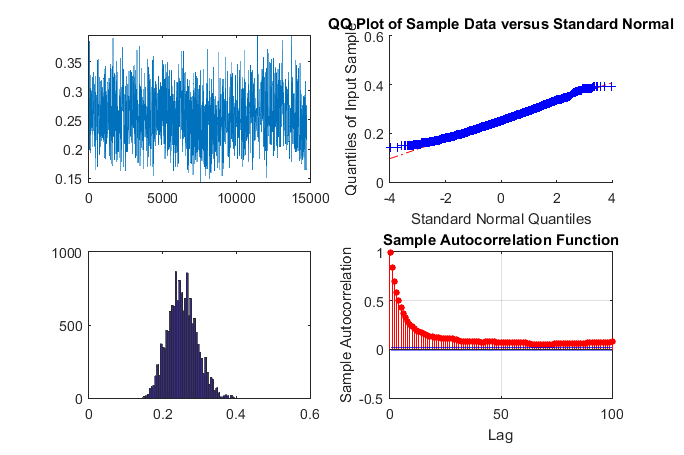
\includegraphics[width = 0.75\textwidth]{sigma_svm}
\caption{Estimation of $\sigma$ with the SVM model $\mathcal{M}_5$}
\label{sigma_svm}
\end{figure}

\section{Determination of the number of particles}
The determination of the correct number of particles $N$ is important in a PMCMC scheme to balance accuracy and good mixing of the chains. The test is based on the knowledge of the true value $\theta_{tr} = \bar{\theta}$. An artificial dataset composed of daily returns with $T=1000$ is generated from model $\mathcal{M}_2$. For a given value of $N$, the bootstrap filter of $\mathcal{M}_2$ is called several times and the variance of the log likelihoods $Var(\log p_N(y|\bar{\theta}))$ is estimated. The process is repeated for different values of $N$. As seen previously in section \ref{sec:tuning_n}, $N$ is optimal when $Var(\log p_N(y|\bar{\theta})) = 0.8464$. From Figure \ref{est_var_pn_theta_n}, $N = 1500$ seems to be the value to select. Pitt (2011) reported that the penalty for a slightly bigger variance is not too severe. The best candidate is therefore $N = 1000$ for $T=1000$. The process is repeated for several values of $T$ to detect a general rule.

\begin{figure}[htb]
\centering
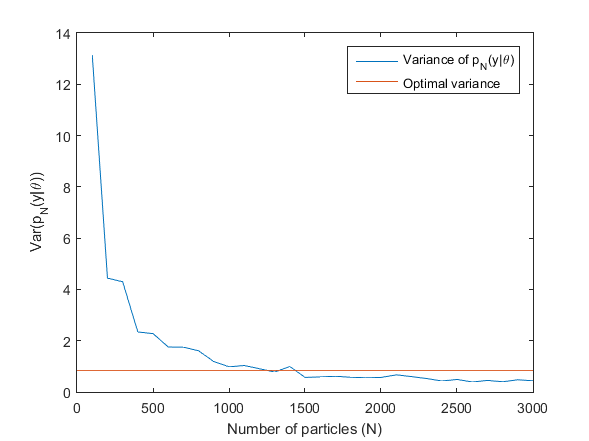
\includegraphics[width = 0.75\textwidth]{tuning_n_optimal_var}
\caption{$Var(\log p_N(y|\bar{\theta}))$ for different values of $N$ on an artificial dataset with $T=1000$}
\label{est_var_pn_theta_n}
\end{figure}

\subsection{Case study with a stock}

\begin{table}[htb]
\centering
\begin{tabular}{llll}
\label{marginal_log_lik_appl}
Parameter    		& $\rho$ & $\sigma$ & $\beta$ \\ 
\hline
Mean            & 0.9981              & 0.2533             & 0.1475\\
Median          & 0.9982              & 0.2514             & 0.1448\\
Max             & 0.9991              & 0.3941             & 0.2189\\
Min             & 0.9865              & 0.1434             & 0.1100\\
Conf Int (95\%) & [0.9904, 0.9989]    & [0.1822, 0.3345]   & [0.1242, 0.1839]\\
Acceptance Rate & 0.08                & 0.14               & 0.11 \\
\hline
\end{tabular}
\caption{Estimation of the parameters for the SV model $\bar{\theta}_{\mathcal{M}5}$. Data is APPL.}
\end{table}

Table \ref{marginal_log_lik_appl} reports estimation for the stochastic volatility models $(\mathcal{M}_1, ..., \mathcal{M}_6)$. $\log (L)$ is the log marginal likelihood $p_N(y|\bar{\theta}, \mathcal{M})$. We find that the Gaussian two factor SV model performs best in terms of the marginal likelihood and AIC criteria. The Kass factor $2 \log BF$ of SVL versus SV is 8 and this indicates strong evidence in favour of the SVL model. Compared to SVt, the Kass factor in favour of SVL is 13 which is also very strong evidence. The distribution of the parameters are also fairly concentrated around their means. The values of $\phi$ very close to one confirm strong daily volatility persistence, in accordance with stylized facts in econometrics known as volatility clustering. The values of $(\phi_X, \sigma_X)$ and $(\phi_Z, \sigma_Z)$ are very interesting. $\phi_X$ is very close to 1 and $\sigma_X$ is very small whereas $\phi_Z$ is almost null and $\sigma_Z$ is high. It means that the volatility of the returns can be decomposed into two distinct processes: a stochastic trend and a process which could be assimilated to white noise. It is easy to see that the stochastic trend process accounts for the volatility clustering and the second process for the noise associated to the returns.



\begin{figure}[htb]
\centering
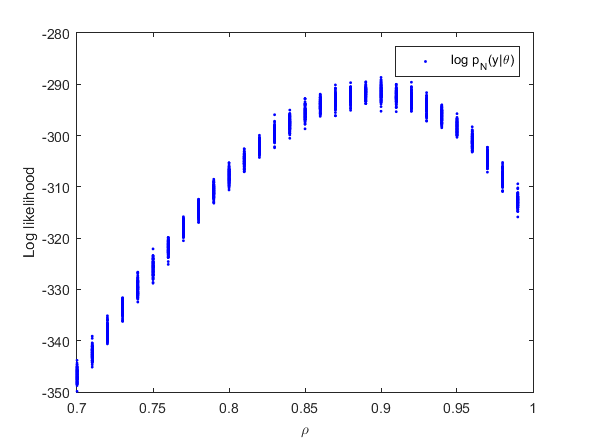
\includegraphics[width = 0.75\textwidth]{tuning_n_rho_varying}
\caption{$\text{Var}(\log p_N(y|\bar{\theta}))$ when $\theta$ varies through $\rho$. Dataset generated from $\mathcal{M}_2$ with $\rho = 0.91, \sigma = 1$ and $\nu = 3$.}
\label{tuning_n_rho_varying}
\end{figure}

\begin{figure}[htb]
\centering
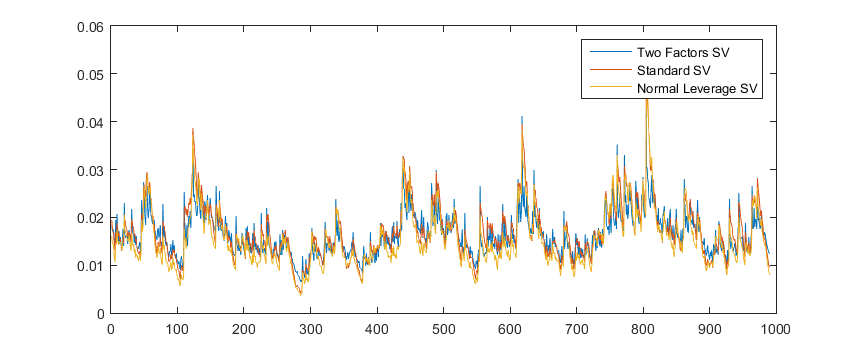
\includegraphics[width = 1\textwidth]{appl_vol_3_models}
\caption{Volatilities of the returns $y_t$ for $\mathcal{M}_1$, $\mathcal{M}_3$ and $\mathcal{M}_6$}
\label{appl_vol_3_models}
\end{figure}

\begin{figure}[htb]
\centering
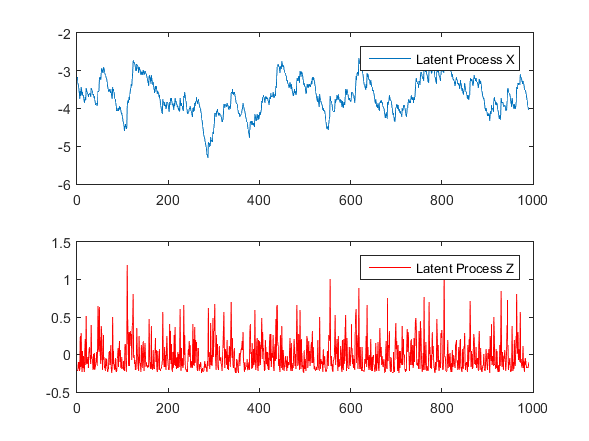
\includegraphics[width = 1\textwidth]{appl_twofactors_latent_processes}
\caption{Estimation of the latent processes $X$ and $Z$ in the Two Factors SV model}
\label{appl_twofactors_latent_processes}
\end{figure}

\begin{figure}[htb]
\centering
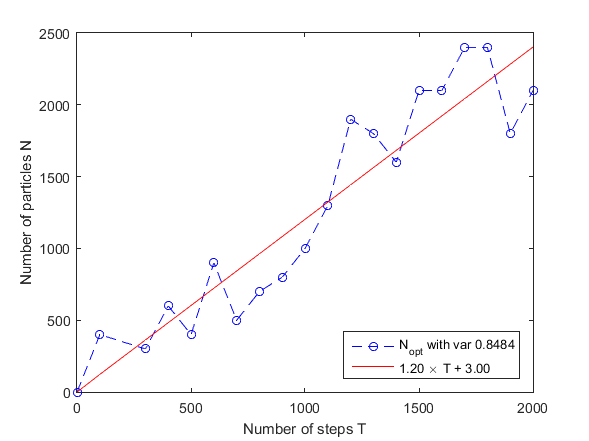
\includegraphics[width = 0.75\textwidth]{n_opt_function_t}
\caption{Behaviour of $N_opt$ when $T$ varies}
\label{n_opt_function_t}
\end{figure}



%put a plot with the stock and all the volatilities of the returns. Can be really interesting.

\subsection{Case study with a spread}

\begin{table}[htb]
\centering
\begin{tabular}{lllllll}
\label{estimation_of_svm_appl}
Parameter        & $\bar{\theta}_{\mathcal{M}1}$ & $\bar{\theta}_{\mathcal{M}2}$ & $\bar{\theta}_{\mathcal{M}3}$ & $\bar{\theta}_{\mathcal{M}4}$ & $\bar{\theta}_{\mathcal{M}5}$ & $\bar{\theta}_{\mathcal{M}6}$\\ 
\hline
$\phi$								                  & 0.9981  & 0.9993 & 0.9986  & 0.9981  & 0.9986 & \\
$\sigma$                                & 0.2238  & 0.1752 & 0.2188  & 0.1694  & 0.2533 & \\
$\beta$                                 & 0.4419  & 0.5722 & 0.4559  & 0.2359  & 0.1625 & 0.3478\\
$\nu$                                   &         & 7.6850 &         &         &         &\\
$\rho$                                  &         &        & -0.3017 &         &         & \\
$\psi$                                  &         &        &         & 0.0060  &         & \\
$\phi_X$                                &         &        &         &         &         & 0.9995\\
$\phi_Z$                                &         &        &         &         &         & 0.1926\\
$\sigma_X$                              &         &        &         &         &         & 0.1268\\
$\sigma_Z$                              &         &        &         &         &         & 0.4913\\
$\mu$                                   &         &        &         &         &         & 0 \\
$\log(L)$                               & 1792.3  & 1797.8 & 1795.1  & 2649.2  & 2649.3  & 1801.3\\
AIC                                     & -3578.6 & -3587.6& -3582.2 & -5290.4 & -5292.6 & -3592.6\\
$2 \log \mathcal{BF}(\cdot, \mathcal{M}6)$& 0     & 0      & 0       & 0       & 0       & 0\\
$N$                                     & 1000    & 1000   & 1000    & 1000    & 1000    & 1000\\
$T$                                     & 689     & 689    & 689     & 689     & 689     & 689\\
Steps                                   & 10000   & 10000  & 10000   & 10000   & 10000   & 10000\\
Burn-in                                 & 1000    & 1000   & 1000    & 1000    & 1000    & 1000\\
\hline
\end{tabular}
\caption{Estimation of the parameters for the SVM model. Data is Spr APPL-MSTA.}
\end{table}

\section{Model selection}

\chapter{Empirical Analysis}
\section{Statistical Arbitrage}
Statistical arbitrage conjectures statistical mis-pricings or price relationships that are true in expectation, in the long run when repeating a trading strategy. Statistical arbitrage is a heavily quantitative and computational approach to equity trading. It describes a variety of automated trading systems which commonly make use of data mining, statistical methods and artificial intelligence techniques. A popular strategy is pairs trade, in which stocks are put into pairs by fundamental or market-based similarities. When one stock in a pair outperforms the other, the poorer performing stock is bought long with the expectation that it will climb towards its outperforming partner, the other is sold short. This hedges risk from whole-market movements. This idea can be easily generalized to $n$ stocks or assets where an asset can be a sector index. The investment strategy we aim at implementing is market neutral, thus we will hold a long and a short position both having the same value in local currency. The difference between this long and short position is known as the spread. Once the spread deviates far from its long-run equilibrium, a position is opened and is unwind when the spread reverts. This approach has the advantage of eliminating the market exposure (memo corr cumsum with SP500 should be around 0).

\section{Composition of the portfolio}
The first motivation of considering a portfolio approach is to lower the volatility associated to each tuple trading by smoothing the net value over time. The approach consists in selection the tuples for trading based on the best in-sample Sharpe Ratios. We form the portfolio of 20 best trading pairs that present the greatest SR in the in-sample simulations and use them to compose a pairs trading portfolio to be employed out-of-sample. Once a trade is initiated, the portfolio is not rebalanced. Only two types of transactions are considered: move into a new position, or the total unwind of a previously opened position. Any opened position is closed at the end of the study.

\section{Bollinger Bands}
\subsection{Framework}
Bollinger Bands is a widely used technical volatility indicator which consists in placing volatility bands $\{Boll^+_t, Boll^-_t\}$ above and below the moving average prices $\{m_t\}$. Volatility is based on the standard deviation, which changes as volatility increases and decreases. The bands automatically widen when volatility increases and narrow when volatility decreases. They are calculated by:

\begin{align*}
m(t) &= \frac{1}{n}\sum_{j=1}^n S_j \text{ (SMA)} \\
Boll^\pm(t) &= m(t) \pm \alpha \sqrt{\frac{1}{n} \sum_{j=1}^n \left(S_j - m(t) \right)}
\end{align*}
where $(S_t)_{t \geq 0}$ is the price of the asset, $n$ is the number of time periods in the moving average and $\alpha$ is the number of standard deviations to shift the Bollinger bands. The default values are $n = 20$ and $\alpha = 2$. $m(t)$ is called the mid band and is used as a relative mean value. $Boll^+(t)$ and $Boll^-(t)$ are respectively the upper and lower bands. Their purpose is to measure how far the price deviates from its mean. Under the assumption that the returns are normally distributed, 95\% of the prices should appear within the bands when $\alpha = 2$. The simple moving averages used in the computation of the bands can be replaced by exponential moving averages which gives more weights to new values and may increase the accuracy.

\begin{figure}[htb]
\centering
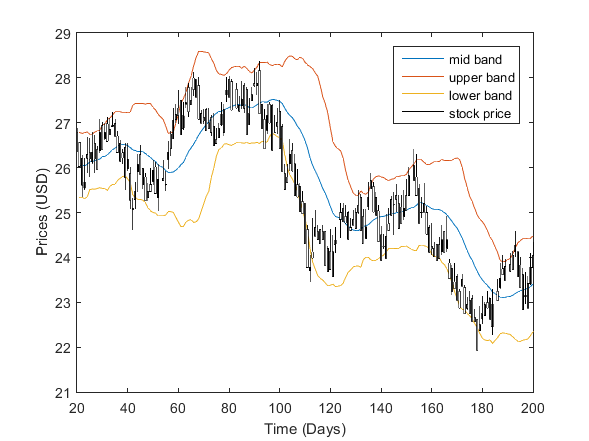
\includegraphics[width = 0.75\textwidth]{bollinger_bands_intro}
\caption{Example of Bollinger bands strategy applied to Walt Disney Co NYSE (2002). The default values are $n = 20$ and $\alpha = 2$.}
\label{bollinger_bands_intro}
\end{figure}
\subsection{Interaction with the SV model}

The SV model is firstly calibrated on the returns $y_t$ of the spread. It is computed as $y_t = \frac{S_t}{S_{t-1}}-1$ where $S_t$ is the spread process.
$x_t$ represents the volatility associated to $y_t$. The log-returns are not used here for a specific reason discussed later. Let's consider the general case where $S_t$ is of the form
\begin{align*}
S_t | \mathcal{F}_{t^-} \sim \mathcal{D}\left( \mu(t), \sigma^2(t) \right)
\end{align*}
where $\mathcal{F}_{t^-}$ contains all the information up to time $t^-$, i.e. the volatility $\sigma(t)$ and the mean $\mu(t)$ are known because the process $x_t$ and $S_{t-1}$ were measured. $\mathcal{D}$ can represent any suitable distribution such as the normal distribution or the $t$-student distribution.
The main idea behind using these stochastic volatility models is to catch the dynamics of the spread through a better estimation of its hidden volatility. A spread is a linear combination of assets where each asset price is one observation of a more general process, over a time interval. From this idea, two main approaches are discussed. \\

\noindent
The first approach consists in working directly with the returns. This contrasts with the default Bollinger bands strategy where the price series is used to compute the volatility. The idea is to detect large movements in returns and bet for a reversion to the long-range mean. This strategy employs a large quantity of trades because it is highly sensitive to price movements. A simple moving average of lag $p$ on the volatility $\sigma(t)$ is considered to detect such movements:
$$SMA_\sigma(t, p) = \frac{1}{p} \sum_{i=0}^{p-1}\sigma(t-i)$$
The mid band is generated from a moving average over the returns. The upper and lower bands are generated by adding and subtracting this rolling volatility $SMA_\sigma$ to the mid band. \\

\noindent
The second method is based on drawing a large of number of sample paths from the model to estimate the volatility of the spread. The volatility computed in this approach is of the same shape as the one computed in the default Bollinger bands strategy. Once every volatility was computed, each of them must be aggregated to form the final rolling volatility $(r\sigma(t)_{t>0}$ from the different generated paths. This quantity is the one used in the computation of the upper and lower bands. The way the rolling volatility is computed and its associated lag are omitted here, for a better clarity. Algorithm 3 summarizes the procedure for the standard stochastic volatility whose equation is given below as a recall
$$S_t | X_t = x_t, S_{t-1} \sim \mathcal{N}(\mu(t) = S_{t-1}, \sigma^2(t)= S_{t-1}^2 \beta^2 \exp(x_t))$$

\begin{algorithm}
\caption{Rolling volatility computed with the standard stochastic volatility model}\label{volatility_std_sv}
\begin{algorithmic}[1]
\Procedure{Input}{$(x_t)_{t>0}$, $(S_t)_{t>0}$, $\theta = \beta$, $N$, $f_a = n^{-1} \sum_{i=1}^N \cdot$}

\For{t from 1 to T}
	\For{i from 1 to N}
		\State Sample the $t^{th}$ value of the $i^{th}$ path, $S_{ti} \sim \mathcal{N}(S_{t-1}, S_{t-1}^2 \beta^2 \exp(x_t))$
	\EndFor{end}
\EndFor{end}
\For{i from 1 to N}
	\State Compute the default rolling volatility $(r\sigma_i(t))_{t>0}$ for the $i^{th}$ path, $(S_{ti})_{t>0}$
\EndFor{end}

\For{t from 1 to T}
	\State $\displaystyle{r\sigma(t) = n^{-1} \sum_{i=1}^N r\sigma_i(t)}$
\EndFor{end}
\\
\Return $(r\sigma(t))_{t>0}$
\EndProcedure
\end{algorithmic}
\end{algorithm}

\noindent
In the most general case, $N$ paths $\{S_{t,n}\}_{0 < n \leq N, t \in \mathbb{N}}$ are generated from an equation involving $S_t | \mathcal{F}_{t^-}$. Let $f_a : \mathbb{R}^{+N} \rightarrow \mathbb{R}^+$ be a positive-definite aggregating function. The aggregated rolling volatility of lag $p$ for all the $N$ paths is defined as $r\sigma(t,p) = f_a(r\sigma(t, p)_1,...,r\sigma(t, p)_N)$.
If $f_a$ is simply the sample mean estimator, the equation is simplified to
$\sigma(t,p) = \frac{1}{N}\sum_{i=1}^N SMA_\sigma(t, p)_i$. It is a well known fact that this estimator is also unbiased and consistent. Depending on the context and on the cross validation phase, $f_a$ can be any measurable function satisfying the conditions above, such as the median or the quantile function.
Note that a rolling volatility is similar to a moving average on the volatility process. When $p \rightarrow 1$, $r\sigma(t,p)$ converges to $\sigma(t)$, the instant volatility associated to $S_t | \mathcal{F}_{t^-}$.

\section{Data}
The data used in this study consists of daily closing prices of the 1232 stocks from the US markets. All the stocks used are listed in stock exchanges such as Dow Jones or NASDAQ, which means they are among the most liquid stocks traded within the US markets. This characteristic is important for the strategies, since it greatly diminishes the slippage effect, reduces the transaction costs and permits to unwind any position without impacting the market too much. The data were obtained from Bloomberg, taken from the period of January 1990 to March 2014. The data are adjusted for dividends and splits, avoiding false trading signals generated by these events, as pointed out by Broussard and Vaihekoski (2012).

\section{Cross Validation}
The whole sample period is divided into sets of length a year. Each set is split into training (in-sample) and testing (out-sample) periods with a ratio of 2:1 (8 and 4 months). The training period is used to select the tradable tuples and to tune the parameters of the strategy. The testing period follows and its purpose is to assess the strategy by running the experiments with the parameters computed in the first period. Cointegration tests are performed for all possible combinations. Of the 1220 stocks, it is possible to form 1.8 billion spreads per period. The resulting cointegrated tuples are then ranked based on the in-sample Sharpe Ratio, similarly to Gatev et al. (2006) and Andrade et al. (2005). After selecting 20 pairs with the highest SR, four months of trading are carried out on the out-sample period. At the end of each trading period, all open positions are closed. The procedure continues in a rolling window fashion until the end of the sample.

\section{Procedure}
A typical trading strategy is made of three parts: selection of the suitable tuples satisfying some criteria like cointegration, create trading signals based on define predefined investment decision rules and finally assess the performance of the strategy.

\subsection{Tuples selection}
It is common in pair trading and more generally in tuple trading to require that the tuples belong to the same sector, for example in Chan (2009) and Dunis et Al. (2010). Other did not adopt this restriction, for example Caldeira Moura (2013). It is harder but nevertheless possible to bypass this restriction at a greater computational cost when the number of assets grows. Several tricks are performed to diminish this combinatorial explosion; one is based on correlation. In the general case, cointegration usually implies correlation but correlation doesn't always imply cointegration. Spurious regression is a very good example where the reverse is not true. The idea is to filter the uncorrelated tuples to limit the number of candidates for cointegration. This assertion holds because a correlation test can be performed much faster than a cointegration test (cf. table 2).

\begin{table}[h]
\centering
\label{table1}
\begin{tabular}{|l|l|l|l|l|}
\hline
Test     & Correlation & Johansen & Aug. Dickey Fuller & Phillips-Perron \\ \hline
Time & 0.33 ms   & 19.08 ms      & 2.33 ms      & 3.04 ms        \\ \hline
\end{tabular}
\caption{Average time spent to test a bivariate time series $X_t = (x_{t1}, x_{t2})$}
\end{table}

\noindent
When it comes to pairs trading, a simple correlation test is enough to conclude. When $n \geq 3$, it is preferred to use the multiple correlation coefficient, better known as $R^2$. It can be computed using the vector $c = (r_{x1y}, r_{x2y},...,r_{xNy})^T$ of correlation $r_{xny}$ between the predictor variables $x_n$ and the target variable $y$, and the correlation matrix $R_{xx}$ of inter-correlations between predictor variables. It is given by $R^2 = c^T R_{xx}^{-1}c$ where $R_{xx}^{-1}$ is the inverse of the matrix

$$R_{xx} =\begin{pmatrix}
r_{x1x1}    & r_{x1x2} & ...  & r_{x1xn}  \\
r_{x2x1}    & \ddots &   & \vdots  \\
\vdots       &   & \ddots &   \\
r_{xnx1}    & \hdots &   & r_{xnxn} \\
\end{pmatrix} $$
One problem arises: the value of the coefficient depends on the ordering of the tuple. To provide convincing evidence of this fact, let's consider a simple example. A regression of $y$ on $x$ and $z$ will in general have a different $R$ that will a regression of $z$ on $x$ and $y$. Let $z$ be uncorrelated with both $x$ and $y$ while $x$ and $y$ are linearly related to each other. A regression of $z$ on $y$ and $x$ will yield a $R$ of zero, while a regression of $y$ on $x$ and $z$ will yield a strictly positive $R$. It means that the ordering inside a tuple has its importance, at least from a statistical point of view. This assertion is also true for all cointegrations tests, except for the Johansen test where the ordering does not matter. This notion of ordering is much less obvious from a pure financial point of view. \\

\noindent
A rigorous testing of cointegration is performed to select the candidates. First, all the time series are tested for a unit root with an Augmented Dickey Fuller test. For a fixed $n$, all possible tuples are formed and $R^2$ is evaluated for each of them. A threshold $R_{th}$ is arbitrary picked up (default is 0.80) and the tuples whose $R^2> R_{th}$ are selected. For every selected tuple, form the spread $\S_t = \beta_0 P_{t0} - \sum_{i=1}^{n-1} \beta_i P_{ti}$ and apply a triple Johansen, Dickey Fuller and Phillips-Perron test to check for cointegration. If the tuple is cointegrated i.e. all the three tests have positive outcome, form the spread and mark it as cointegrated.

\subsection{Creation of the Trading Signals}
For cointegrated marked spreads, the second part of the algorithm creates trading signals based on predefined investment decision rules. A trading rule determines when to open and close a position. With Bollinger bands strategy, the basic rule is:

\begin{itemize}
\item Open a long position when there is an upward crossing between the spread and the lower band;
\item Unwind (close) this position when there is an upward crossing between the spread and the upper band;
\item Open a short position when there is a downward crossing between the spread and the upper band;
\item Unwind this position when there is a downward crossing between the spread and the lower band.
\end{itemize}
Empirical studies showed that this strategy is one of the most profitable with the use of Bollinger Bands. When a long position is initiated, the first asset is bought with quantity 1 and the remaining assets of the tuple are sold with the respective quantities indicated by the cointegrated vector $\beta$. It is assumed that the trader can buy a portion of an asset. This same position is closed by selling one unit of the first asset and buying the remaining assets, still in the same proportions.

\subsection{General parameters of the strategy}
Throughout the strategies, we consider 0.5\% of the total nominal as transaction costs for tuple trading. This choice was discussed for pairs trading in Dunis et al. (2010), Dunis \& Ho (2005) and Alexander \& Dimitriu (2002). For simplicity, no rental costs are considered for short positions but the capital invested in short selling cannot exceed 50\% of the total capital, invested or in cash. The asset allocation in the portfolio follows a invested weighting scheme with no dynamic rebalancing. Each tuple is given the same weight throughout the study. If there are no open positions, the money is not invested and remain as cash in the portfolio. For a particular tuple, the number of open positions is limited to only one on the spread. The strategy is self-financing, i.e. profits are reinvested and no deposits or withdrawals are permitted.

\subsection{Optimization of the strategy}

Bollinger bands strategy requires to estimate three parameters: the number of periods $p$ to compute the bands, the type of moving average used in the mid band and $\alpha$ which controls the interval between the volatility bands. John Bollinger suggests $p = 20, \alpha = 2$ and simple moving average by default. To optimize those parameters, a cross-validation scheme is performed. The criterion of optimization is the in-sample Sharpe Ratio.

\subsection{Performance Assessment}
The performance of the portfolios are examined in terms of cumulative return, variance of returns $(\sigma^2)$, Sharpe Ratio (SR) and Maximum Drawdown (MDD). The maximum drawdown (MDD) is defined as the maximum percentage drop incurred from a peak to a bottom up to time $T$. Drawdowns help determine an investment's financial risk.

$$MDD(T) = \smash{\displaystyle\max_{\tau \in (0,T)}} \left[\smash{\displaystyle\max_{\tau \in (0,T)}} X(t) - X(\tau) \right] $$

The Sharpe Ratio (RP) based on daily returns is defined as

$$SR =  \sqrt{252 }  . \frac{\bar{R_t}}{\sqrt{T^{-1} \sum_{t=1}^T (R_t - \bar{R_t})^2 }} \text{, where } \bar{R_T} = T^{-1} \sum_{t=1}^T R_t $$

One of the techniques to assess the performance of a strategy is to compare it to the very simple Buy and Hold strategy where the holder buys various assets at time $0$ and keep them until time $T$. Gatel et Al (2006) also considered a bootstrap approach to generate random trading signals to assess the performance of a strategy over pure randomness. This approach is not discussed here since such a strategy has a negative expectation because of the trading costs and assuming the fact that you cannot beat the market with a random approach in the long run. So better not trade at all in this case.

\section{Estimation and out-of-sample results}
The sample is split into several training (in-sample) and testing sets (out-of-sample). Cross validation is performed on the training sets to tune the parameters of the strategies. The performance is evaluated on the testing set. We suggest a period of one year for testing and four months for testing.

\section{Presentation of the dataset}
The sample period used starts in January 1990 and ends in March 2014 summing up to 8844 observations. Daily equity closing prices obtained from Bloomberg. The analysis covers all stocks in the SP500 index from the American stock markets. The proposed statistical arbitrage generated average excess returns of 12\% per year in out-of-samples simulations, Sharpe ratio of 1.70, low exposure to the equity market and relatively low volatility and 5pt basis for transaction costs. Even in market crashes, it turns out that the strategy is still highly profitable, reinforcing the usefulness of co-integration in quantitative strategies.

\section{Model selection}
For each training period, the spread is computed and all the stochastic volatility models presented are applied to its returns. The model with the highest marginal likelihood is taken as reference and the Bayes factors are computed relatively to this model. AIC is also used to reinforce our decisions. We set $N$, the number of particles to 1000 and run the different samplers for $M = 10000$ Metropolis Hastings iterations. After discarding the first 1000 iterations, we collect the final sample and compute the posterior mean $\bar{\theta}$, the posterior median, 95 \% credibility intervals, the log likelihoods that results from the particle filter, the logarithm of the marginal likelihood, the AIC criterion and the M-H acceptance ratio. We find that the Gaussian Stochastic Volatility Leverage model performs best in terms of the marginal likelihood criterion. An advantage of using Bayes Factors and AIC is that they automatically penalize highly parametrized models that do not deliver improved content. Figure 1 displays the SPX500 index for the period 1/1/2010-1/1/2014 followed by the returns and the filtered estimates of $(X_t)_{t>0}$.
We find that the Gaussian SVL model performs best in terms of the marginal likelihood and AIC criteria. The Kass factor $2 \log BF$ of SVL versus SV is 8 and this indicates strong evidence in favour of the SVL model. Compared to SVt, the Kass factor in favour of SVL is 13 which is also very strong evidence. The distribution of the parameters are also fairly concentrated around their means. The values of $\phi$ very close to one confirm strong daily volatility persistence, in accordance with stylized facts in econometrics known as volatility clustering.

\section{Heston}
\subsection{Simulation of Probability Densities}
By Ito calculus, and more precisely the Euler-Maruyama method, the Heston stochastic process can be discretized and results in:

\begin{align*}
S_t &= S_{t-1} + r S_{t-1} dt + \sqrt{V_{t-1}}S_{t-1} \sqrt{dt}Z_t^S \\
V_t &= V_{t-1} + \kappa(\theta - V_{t-1})dt + \sigma \sqrt{V_{t-1}} \sqrt{dt} Z_t^V
\end{align*}
where the innovations $\{Z_t^S\}_{t \geq 0}$ and $\{Z_t^V\}_{t \geq 0}$ are standard normal random variables with correlation $\rho$. The generation is made simple by considering the Cholesky decomposition,

\begin{align*}
Z_t^S &= \phi_t^S \\
Z_t^V &= \rho \phi_t^V + \sqrt{1-\rho^2} \phi_t^V
\end{align*}
where $\{\phi_t^S\}_{t \geq 0}$ and $\{\phi_t^S\}_{t \geq 0}$ are independent standard normal random variables.
%%%% http://math.nyu.edu/~atm262/fall06/compmethods/a1/nimalinmoodley.pdf p36

\section{Z-score}
Once the spread $(\epsilon_t)_{t \geq 0}$ is formed, Caldeira Moura (2013) suggests to compute the dimensionless z-score. Defined as $z_t = \frac{\epsilon_t-\mu_\epsilon}{\sigma_\epsilon}$, it measures the distance to the long-term mean in units of long-term standard deviation. The basic rule is to open a position when the z-score hits the n-quantile of the standard normal distribution $\Phi^{-1}(q_n)$. According to the 68-95-99.7 rule, having a two standard deviation thresholds from above and below seems relevant. If the z-score hits the low threshold, it means that the spread is underpriced and a long position should be opened. When the spread reverts to its mean, the position has to be unwind. The same reasoning for the high threshold holds for short positions. Caldeira Moura (2013) suggested the basic trading strategy signals:

\begin{align*}
\text{Open long position if } &\leq \Phi^{-1}(q_{OL}) = -2.00\\
\text{Open short position if } &\geq \Phi^{-1}(q_{OS}) = 2.00\\
\text{Close short position if } &\leq \Phi^{-1}(q_{CS}) = 0.75\\
\text{Close long position if } &\geq \Phi^{-1}(q_{CL}) = -0.50
\end{align*}

\section{Results}

The strategy is compared to the traditional buy and hold strategy where the investor buys a basket of stocks to reproduce the S\&P500 index and holds it until the end of the period where the position is unwound. Table xx presents the results of both strategies.

\begin{table}[htb]
\centering
\begin{tabular}{lll}
\hline
Summary Statistics of the tuple Trading strategy				& Strategy & SPX (Buy and Hold)\\ \hline
\# of observations in the sample								& 8844  \\
\# of observations in the training window						& 170 \\
\# of days in the trading period								& 84 \\
\# of trading periods											& 1\\
\# of pairs in each trading period   							& 20\\
\# min of cointegrated pairs in a trading period 				& 35000\\
\# max of cointegrated pairs in a trading period 				& 35000\\
Average annualized return 										& 14.88\% \\
Annualized volatility 											& 6.92\% \\
Annualized Sharpe Ratio 										& 2.54  \\
Largest daily return 											& 2.80\% \\
Lowest daily return 											& -1.94\% \\
Cumulative profit 												& 844.48\%\\
Correlation with the market returns 							& 0.061\\
Skewness														& 1.09\\
Kurtosis 														& 19.89\\
Maximum Drawdown  												& 3.80\% \\
\hline
\end{tabular}
\end{table}

\noindent
Figure xx compares the cumulative excess returns and volatility of the strategy with the ones of the SPX index. The portfolio composed of the tuples shows very little volatility compared to the Buy and Hold strategy of the S\&P500 index. The second panel presents the implied volatility of the returns for both strategies computed with a standard stochastic volatility model. The strategy accounts for a low and stable volatility for the whole period. A very low correlation with the market returns attests the market neutral property of the strategy. Table 3 shows the performance year by year of the strategy and it is worth noticing that the excess returns is very high during the crisis where the volatility was very high. As highlighted by Khandani \& Lo (2007) and Avellaneda \& Lee (2010), the second semester of 2007 and first semester of 2008 were quite complicated for quantitative in vestment funds. Particularly for statistical arbitrage strategies that experienced significant losses during the period, with subsequent recovery in some cases. Many managers suffered losses and had to deleverage their portfolios, not benefiting from the subsequent recovery. We obtain results which are consistent with Khandani \& Lo (2007) and Avellaneda \& Lee (2010) and validate their unwinding theory for the quant fund drawdown. Note that in Figure 3, the proposed pairs trading strategy presented significant losses in the first semester of 2008, starting its recovery in the second semester. Khandani \& Lo (2007) and Avellaneda \& Lee (2010) suggest that the events of 2007-2008 may be a consequence of a lack of liquidity, caused by funds that had to undo their positions. \cite{delmoral2004}

%\begin{figure}[!htb]
%\centering
%\includegraphics[width = 1\textwidth]{img/optimal_lag.pdf}
%\caption{Spread ALCOA INC, AVERY DENNISON CORP, BANK OF NEW YORK MELLON CORP 23-Jun-1995 - 27-Apr-2002}
%\label{fig:1}
%\end{figure}

%\begin{figure}[!htb]
%\centering
%\includegraphics[width = 1\textwidth]{img/profiling_n.pdf}
%\caption{Profiling the number of particles $N$ for $T = 1000$}
%\label{fig:1}
%\end{figure}

%\begin{figure}[!htb]
%\centering
%\includegraphics[width = 1\textwidth]{img/smoothed_var_rho.pdf}
%\caption{Profiling the variance $p_N(y|\theta)$ for several $\rho$ and $N=1000$}
%\label{fig:1}
%\end{figure}

It converges to the standard normal probability density function as $\sigma \rightarrow 0$.

%\begin{figure}[!htb]
%\centering
%\includegraphics[width = 1\textwidth]{img/expnorm.pdf}
%\caption{$\exp \left(\frac{\sigma}{2} \epsilon_R \right) \epsilon_R \text{, } \epsilon_R \sim N(0,1) \text{, } \sigma > 0$}
%\label{fig:1}
%\end{figure}

\cleardoublepage
\phantomsection
\addcontentsline{toc}{chapter}{\bibname} % Add an entry for the Bibliography in the Table of Contents
%\pagestyle{headings}
\bibliographystyle{abbrvnat} % set the bibliography style
\bibliography{bibtexfile} % generate the bibliography
%\bibliographystyle{abbrvnat} % <- Mistake in earlier version. After the bibliography is created it's too late to change the style.
% Pick a sensible bibliography style. 
% If like above you choose to use author-year style citations, you must choose a natbib-compatible bibliographystyle such as 'plainnat'. Abbrvnat is one of the few built-in styles of this type. You may find many more bibliography styles (*.bst files) online. You can also choose to write your bibliography manually instead of using BibTeX (This will take you longer, unless you plan to use the content of a BibTeX-generated *.bbl file as your starting point).
% When creating a BibTeX file using e.g. reference manager software, note that the entries may contain additional unwanted fields which you would then need to erase. For example, you probably don't want to include the URL of a journal paper in your bibliography.


%\cleardoublepage \fancyhead[L]{APPENDIX}
 % This line declares that you are starting the appendix.
% If you want a single Appendix and want it to be called Appendix instead of Appendix A, the following should work:
%\setcounter{secnumdepth}{-1} %This turns off automatic chapter numbering
%\chapter{Appendix}

\chapter{Appendix}

\section{Stratified Resampling}
\lstinputlisting{../../filters/resampleStratified.m}

\section{Bootstrap Particle Filter for Standard SV}
\lstinputlisting{../../filters/BootstrapParticleFilter.m}

\section{Bootstrap Particle Filter for Student SV}
\lstinputlisting{../../filters/BootstrapParticleFilter_Student.m}

\section{Bootstrap Particle Filter for Normal Leverage SV}
\lstinputlisting{../../filters/BootstrapParticleFilter_NormalLeverage.m}

\section{Bootstrap Particle Filter for Two Factors SV}
\lstinputlisting{../../filters/BootstrapParticleFilter_TwoFactors.m}

\section{Particle Markov Chain Monte Carlo (Abstract Class)}
\lstinputlisting{../../pmcmc/ParticleMarkovChainMonteCarlo.m}

\section{Particle Markov Chain Monte Carlo Standard Stochastic Volatility Model}
\lstinputlisting{../../pmcmc/ParticleMarkovChainMonteCarloSV.m}

\section{Particle Markov Chain Monte Carlo SV Normal Leverage Model}
\lstinputlisting{../../pmcmc/ParticleMarkovChainMonteCarloSVNormalLeverage.m}

\section{Particle Markov Chain Monte Carlo SV Student Model}
\lstinputlisting{../../pmcmc/ParticleMarkovChainMonteCarloStudentBetaSV.m}

\section{Particle Markov Chain Monte Carlo SV Two Factors}
\lstinputlisting{../../pmcmc/ParticleMarkovChainMonteCarloSVTwoFactors.m}

\section{Bayes Factor - Kass and Raftery}
\lstinputlisting{../../likelihoods/BayesFactor.m}

\section{Marginal Likelihood $p(y_{1:T})$ - Gelf and Dey}
\lstinputlisting{../../likelihoods/GelfandDey_LogMarginalY.m}

\section{Spread Finder}
\lstinputlisting{../../coint/deepsearch/SpreadFinder.m}

\section{Spread Constructor}
\lstinputlisting{../../coint/deepsearch/SpreadConstructor.m}

\section{Build Order}
\lstinputlisting{../../coint/deepsearch/SpreadBuildOrder.m}

\section{Trading Strategy}
\lstinputlisting{../../coint/deepsearch/SimpleTradingStrategy.m}

\section{Trading Strategy Cross Validation}
\lstinputlisting{../../coint/deepsearch/SimpleTradingStrategyCV.m}

\section{Reversion Frequency Calculator}
\lstinputlisting{../../coint/deepsearch/ReversionFrequencyCalculator.m}

\section{Crossing Points Calculator}
\lstinputlisting{../../coint/deepsearch/CrossingPointsCalculator.m}

\section{Main}
\lstinputlisting{../../coint/deepsearch/Main2.m}

\end{document}
